\clearpage

\section{线性空间与线性映射}

\subsection{线性空间}

\subsubsection{例子与概念}

在$n$维向量空间$\mathbb{K}^n$中，
“向量”被规定为$n$维数组.
这种规定固然方便，
但是如果把它当作对于“向量”概念的分析，
却不太令人满意.
事实上，如果抛开一切语境来问“向量是什么？”，
似乎有点难回答.
我们一般会认为，
“向量”应当是一些能做加法和数乘，
可以反映方向性质的一类东西.
但是上述要求可以被各式各样的数学对象所承载，
并不限于$n$维数组.
以下略举几例，
请体会它们是否承载了我们熟悉的$\mathbb{R}^2$所描述的向量的性质：\medskip

\textbf{例1}~~\textit{根据高中平面向量的观念定义所谓“几何向量”：把平面中的箭头（有向线段）称为向量，
箭头之间可以按平行四边形法则做加法，用实数$k$的数乘代表箭头的（有向）长度变为原来的$k$倍.
任意两个不共线的箭头都可以唯一地线性表示出每个箭头.}\medskip

\textbf{例2}~~\textit{复数域$\mathbb{C}$. 任何一个复数$z$可以表示为$a + bi$，
其中$a,b \in \mathbb{R}$，分别称为$z$的实部和虚部.
$z$可以看成$1$与$i$的线性组合，
$a$和$b$是组合系数.
两个复数$z_1 = a_1 + b_1 i$和$z = a_2 + b_2 i$之间的加法规定为$z_1 + z_2 = (a_1 + a_2) + (b_1 + b_2)i $，
复数$z = a+ bi$被实数$k$数乘规定为$kz = ka + kbi$.
可以把复数用箭头的形式表示在复平面上，
则复数加法和数乘的几何意义就是箭头的加法和数乘.}\medskip

\textbf{例3}~~
\textit{线性方程组$A_{m \times n} \bm{x} = \bm{0}$的解集$\operatorname{Ker} A$，其中$\mathrm{rank}(A)=n-2$.
我们此前证明过，
$\operatorname{Ker}\mathcal{A}$是$\mathbb{K}^n$的一个$2$维子空间.
可以取出$2$个线性无关的向量$\bm{\xi}_1,\bm{\xi}_2$作为基础解系，
并给出通解的形式$c_1 \bm{\xi}_1 + c_2 \bm{\xi}_2,~ c_1 ,c_2 \in \mathbb{K}$.
}\medskip

上述$3$例，
虽然表现形式差异很大，
但似乎都能作为“平面向量”的实体来看待.
以下继续给出$3$个例子，
它们乍看与“向量”没什么关系，
但是细想之下，
其实相似之处极多.\medskip

\textbf{例4}~~
\textit{常系数齐次线性微分方程$y'' + y = 0$的通解.
在高等数学中曾经证明过，
该方程的任意两个解相加，或者一个解乘以实数$k$，
仍然是该方程的解（即解集对加法和数乘封闭）.
可以写出方程的通解$C_1 \sin x + C_2 \cos x$.
其中，$\sin x $和$\cos x$是方程的两个线性无关的特解，
称为基本解组.
}\medskip

\textbf{例5}~~
\textit{电子的自旋量子态.
在特定方向上测量一个电子的自旋，
结果可能为上旋或者下旋，分别记为$\ket{\uparrow}$
和$\ket{\downarrow}$.
这两种状态是电子在该方向上自旋的本征态.
当一个电子未被测量时，
它的自旋状态可以被表示为本征态的一个特定的线性组合，
即所谓量子叠加态$\lambda_1 \ket{\uparrow} + \lambda_2 \ket{\downarrow}$，
其中$\lambda_1 , \lambda_2 \in \mathbb{C}$.
}\medskip

\textbf{例6}~~
\textit{$\mathbb{R}$上不超过$1$次的多项式集合$\mathbb{R}_1 [x]$.
其中的每个元素$f(x)$可以表示为$ax + b$，其中$a ,b \in \mathbb{R}$.
$\mathbb{R}_1[x]$中的加法和数乘即是多项式的加法和数乘.
确定$\mathbb{R}_1[x]$中的元素只需确定一次项系数$a$和常数项$b$.
换句话说，
$\mathbb{R}_1[x]$中的元素可以看成$x$与$1$的线性组合，
$a$和$b$是组合系数.
}\medskip

用心体会这$6$个例子与$\mathbb{R}^2$的共同点，
你可能感觉到所有这些例子从某种角度上可以说是“本质没有区别”的.
具体有哪些共同点呢？
不妨停下来想一想，
再看是否和我总结的一样：\medskip

(1)~~在某个集合$V$中，
规定了\textbf{加法}和\text{数乘}两种运算.
注意数乘需要使用到$V$之外的“数”，
因此需要给$V$指派一个\textbf{数域}$\mathbb{K}$作为数乘所用的“数”.
上述大部分例子中指派的数域都是$\mathbb{R}$，
只有例5使用的是$\mathbb{C}$.
加法和数乘对于集合$V$必须是\text{封闭}的.

(2)~~可以选出$V$中$2$个\textbf{线性无关}的元素
（请自行回顾“线性无关”的含义），
$V$中的任何一个元素都能唯一地表示为它们的线性组合.
因此，这$2$个元素在$V$中扮演了基础性的角色.
无论是线性方程组的“基础解系”，
齐次线性微分方程的“基本解组”，
还是粒子的“本征态”，
都体现了类似的观念.
这实际上就是为$V$找到了一组\text{基}.\medskip

对于加法和数乘上的共同点，
需要思考地更深入一些.
形式化地说，
所谓加法就是$V \times V \to V$的二元映射，
所谓数乘就是$\mathbb{K} \times V \to V$的二元映射.
但是，
所谓的“二元映射”浩如烟海，
其中许多连加法结合律，加法交换律之类最基本的运算规律都不满足，
这当然不符合我们对“向量”的要求.
因此，
我们需要对向量的运算性质做一些基本的规定.
事实上，在$\mathbb{K}^n$中，
我们曾经总结过$8$条运算性质
（请先自行回顾，在后文会重新列举一遍）.
这正是我们现在所需要的.\medskip

经过以上的思考，
我们把众多例子的共同点给刻画了出来.
这就自然地引出了\textbf{线性空间}的定义.
可以认为这是对“向量”的一种更抽象也更泛用的定义.
\medskip

\textbf{线性空间的定义}~~
\textit{设$V$是一个集合.
为它指派一个数域$\mathbb{K}$，
并在$V$中定义元素之间的加法和数乘，
满足以下$8$条规则，
那么称$V$是数域}\textbf{$\mathbb{K}$上的线性空间}
\textit{，$V$中的元素称为}\textbf{向量}：

(1)~\textbf{加法单位元：}\textit{$V$中存在唯一的零元素$\bm{0}$，
使得对任意$\bm{x} \in V$，$\bm{0} + \bm{x} = \bm{x}$. }

(2)~\textbf{加法结合律：}\textit{$\bm{x}_1 +( \bm{x}_2 + \bm{x}_3) = (\bm{x}_1 + \bm{x}_2) + \bm{x}_3$，$\forall \bm{x}_1,\bm{x}_2, \bm{x}_3 \in V$.}

(3)~\textbf{加法的逆：}\textit{$\forall \bm{x} \in V$，存在一个它的“负元素”$-\bm{x}$，使得$\bm{x}+(-\bm{x}) = \bm{0}$.}

(4)~\textbf{加法交换律：}\textit{$\bm{x}_1 + \bm{x}_2 = \bm{x}_2 + \bm{x}_1$，$\forall \bm{x}_1,\bm{x}_2 \in V$.}

(5)~\textbf{数乘单位：}\textit{$1 \cdot \bm{x} = \bm{x}$，$\forall \bm{x} \in V$.}

(6)~\textbf{数乘结合律：}\textit{$k(l \bm{x}) = (kl)\bm{x}$，$\forall k,l \in \mathbb{K}$，$\bm{x} \in V$.}

(7)~\textbf{数乘分配律I：}\textit{$k (\bm{x}_1 + \bm{x}_2) = k \bm{x}_1 + k \bm{x}_2$，$\forall k \in \mathbb{K}$，$\bm{x_1},\bm{x_2} \in V$.}

(8)~\textbf{数乘分配律II：}\textit{$(k+l)\bm{x} = k \bm{x} + l \bm{x}$，$\forall k,l \in \mathbb{K}$，$\bm{x} \in V$.}\medskip

按此定义，
之前给出的所有$6$个例子全都是线性空间.
其中，电子的自旋量子态构成$\mathbb{C}$上的线性空间，
其余是$\mathbb{R}$上的线性空间.

关于线性空间的概念做几条注记：
\medskip

(1)~~我们对线性空间中的元素“长得如何”是只字不提的，
无所谓它是箭头、数组，甚至是函数、多项式、量子态等等.
即：
我们不会用“向量长什么样”的方式来回答“向量是什么”的问题，
而是会说“向量是满足xxx性质的一类数学对象”.
至于箭头、数组、量子态等都是向量的具体例子.
这种观点相比以前更加抽象，
但是抓住了向量最本质的特点.

(2)~~中学阶段认为，向量是一种“既有大小又有方向”的量.
但是现在把向量看作线性空间的元素，
这说法就是完全错误的了.
所谓大小、长度等概念，
在线性空间中称为\textbf{范数}；
“方向”则是由\textbf{内积}给出
（即计算向量的“夹角”）.
然而线性空间的定义本身并没有给出向量的范数和内积，
它们是需要额外附加的装备.
例如，
目前我们知道例4中的函数集合$C_1 \sin x + C_2 \cos x$构成线性空间，
此时谈论函数的“大小”和“方向”似乎是毫无意义的，
必须在指定了范数和内积结构之后才能谈论
（参见高等数学傅里叶级数章节）.

(3)~~线性空间定义中的$8$条规则如同线性空间中的“公理”，
其他我们所熟知的向量运算性质，
即使看起来十分显然，
也不是天生就有的，
需要通过这$8$条规则证明出来.
比如，
可以尝试证明$0 \cdot \bm{x} = \bm{0}$，
$(-1) \cdot \bm{x} = -\bm{x}$.

(4)~~注意区分数域$\mathbb{K}$中的数$0$与线性空间$V$中的零元素$\bm{0}$（零向量）.
也许在某些情况下你会忘记这种区分，
比如把$\mathbb{C}$看作$\mathbb{R}$上的线性空间时，
$\mathbb{C}$中的$0$和$\mathbb{R}$中的$0$一样吗？
按线性空间的定义来说是不一样的.
同理，也要注意区分数域中的加法乘法与线性空间中的加法和数乘.
不同的线性空间的加法和数乘亦有不同，
但习惯上都以$+$和$\cdot$（常常省略）表示，
需要特别小心.

(5)~~在线性代数中，
大部分结论与线性空间所配套的数域$\mathbb{K}$无关（例如第二章中讲到的内容），
甚至换成更一般的域$F$也成立.
因此我们经常省略数域$\mathbb{K}$不提，


(6)~~第一次接触线性空间这种抽象化概念可能有陌生感.
其实它的性质和向量空间$\mathbb{K}^n$完全没有区别，
只不过“向量”的表现形式不同而已.
接下来的小节将详细解释这一点.


\subsubsection{重要概念复习}

之前在$\mathbb{K}^n$中讨论过的许多概念
都可以照搬进一般的线性空间中讨论，
只不过把“$\mathbb{K}^n$中的元素”替换为
“线性空间$V$”中的元素.
作为复习，
这里把概念的定义重新写一遍.
\medskip

\textbf{线性子空间}~~
\textit{设$V$是线性空间，$V_0$是$V$的一个子集.
如果$V_0$对$V$中规定的加法和数乘封闭，则称$V_0$是$V$的一个线性子空间，简称子空间}.

注1：该定义其实就是要求$V_0$作为线性空间$V$的子集也是一个线性空间.

注2：$\{ \bm{0} \}$与$V$都是$V$的线性子空间，
它们分别是$V$的最小和最大的子空间，
称为平凡子空间.

注3：线性子空间$V_0$的加法和数乘必须是从$V$直接继承而来，
而不是为$V_0$规定一种不同于$V$中的加法和数乘运算.\medskip

\textbf{线性相关/线性无关}~~
\textit{线性空间$V$中的向量组$\bm{\alpha}_1 , \bm{\alpha}_2 , \cdots , \bm{\alpha}_s~(s \ge 1)$是线性相关的，
当且仅当有数域$\mathbb{K}$中的一组不全为$0$的系数$k_1 , k_2 , \cdots , k_s$，使得}
\begin{eq1}
    k_1 \bm{\alpha}_1 
    + k_2 \bm{\alpha}_2 
    + \cdots 
    + k_s \bm{\alpha}_s 
    = \bm{0} \end{eq1}
\textit{反之，如果上式成立可以推出系数$k_1 , k_2 , \cdots , k_s$全为$0$，那么称该向量组是线性无关的.}
\medskip

\textbf{极大线性无关组}~~
\textit{设$\{ \bm{v}_1 , \bm{v}_2 , \cdots , \bm{v}_s \}$是线性空间$V$的一个向量组.
如果它的一个部分组本身是线性无关的，
但是从向量组的其余向量（如果还有的话）中任取一个添进去，
得到的新部分组都线性相关，
称它是一个极大线性无关组.}

注：一个向量组的极大线性无关组的向量个数是唯一的，
这一点并不那么显然.
详见第二章的讨论.\medskip


\textbf{线性空间的基}~~
\textit{把整个线性空间$V$看成一个无穷向量组，它的一个极大线性无关组就是线性空间$V$的一组基.
展开来说，
$V$中的一个向量组要成为$V$的一组基当且仅当以下两个条件都满足：
(1)~~该向量组线性无关；
(2)~~该向量组能线性表示$V$中的每个向量.
}\medskip

\textbf{线性空间的维数}~~
\textit{线性空间$V$的一组基的向量个数称为$V$的维数，记作$\text{dim}~V$}.

注：在线性代数中，默认只讨论有限维的线性空间.


\subsubsection{向量的坐标表示}

对于任意的$n$维线性空间$V$，
都能选取它的$n$个线性无关向量作为一组基，
用它线性表示$V$中的每个向量，
且表示方法唯一.
这是我们之前总结的线性空间的重要共同点.

我们在中学阶段会用解析几何的办法把几何问题给代数化，
基本方法是建立平面/空间直角坐标系，
把几何上的点（向量）用坐标来表示，
极大地方便了计算.
\textbf{所谓坐标，其实就是$\mathbb{K}^n$中的元素}
（中学的平面坐标是$\mathbb{R}^2$中的元素，
空间坐标是$\mathbb{R}^3$中的元素）.
在线性代数中，
我们又学习了矩阵和行列式等工具，
它们把线性映射和向量的问题归结到数域$\mathbb{K}$中进行计算.
我们自然希望在一般的线性空间$V$中使用这些工具.
第一步便是设法把$V$中元素表示成\textbf{坐标}.

设$V$是$n$维线性空间，
$\{ \bm{e}_1 , \bm{e}_2 , \cdots , \bm{e}_n \}$是$V$的一组基.
任取$V$中的一个向量$\bm{\alpha}$，
则它可以唯一地用这组基线性表示：
\begin{eq1}
    \bm{\alpha} = x_1 \bm{e}_1 + x_2 \bm{e}_2 + \cdots + x_n \bm{e}_n \end{eq1}

所谓“唯一”，
就是说如果给定$\{ \bm{e}_1 , \bm{e}_2 , \cdots , \bm{e}_n \}$这组基，
线性表示的系数$(x_1 , x_2 , \cdots , x_n)$对$\bm{\alpha}$来说是唯一的.
我们把这组系数称为$\bm{\alpha}$\textbf{在这组基下的坐标}.
这样，
对于$n$维线性空间$V$里的每个元素，
都能唯一地给它分配一个坐标.
同一个向量不可能拥有两个不同的坐标，
每一个坐标也必定对应了某个向量.
以上的事实用更形式化的方式来描述是这样的（这个描述很重要）：

对于数域$\mathbb{K}$上的$n$维线性空间$V$，
给定了它的一组基$\{ \bm{e}_1 , \bm{e}_2 , \cdots , \bm{e}_n \}$，
那么我们会有$V \to \mathbb{K}^n$的一个双射$\varphi$（可以非正式地称它为“坐标映射”），
它的映射规则如下：
\begin{eq1}
     \bm{\alpha} = a_1 \bm{e}_1 + a_2 \bm{e}_2 + \cdots + a_n \bm{e}_n
     \mapsto (a_1 , a_2 , \cdots , a_n)  \end{eq1}

即我们用$\varphi (\bm{\alpha})$表示$\bm{\alpha}$在基$\{ \bm{e}_1 , \bm{e}_2 , \cdots , \bm{e}_n \}$下的坐标.
坐标为研究线性空间提供了必要的计算工具.
不久之后我们会学习如何用$\mathbb{K}^n$中的工具计算线性映射和基变换等等.
但是在开始动手之前，
需要解决一些理论问题.

首先，
我们提出坐标的概念是希望线性空间$V$中向量的运算可以转化到$\mathbb{K}^n$中完成，
如何确保这种“转化”是合理的？
我们已经知道坐标映射$\varphi$是一个双射.
但这个说法还不全面.
我们以一个简单的情形为例：
$2$维线性空间$V$中的$2$个向量$\bm{\alpha}$和$\bm{\beta}$.
假设它们在基$\{\bm{e}_1 , \bm{e}_2 \}$下的坐标$\varphi (\bm{\alpha})$和$\varphi (\bm{\beta})$分别是$(a_1 , a_2)$和$(b_1,b_2)$.
你能够立即说出向量$\bm{\alpha}+\bm{\beta}$的坐标是$(a_1 + a_2 , b_1 + b_2)$，
向量$k\bm{\alpha}$的坐标是$(ka_1 , ka_2)$——
这些计算是如此顺手以至于你可能都忘了这是从$\varphi$的定义推出来的：
\begin{eq1}
    \varphi (\bm{\alpha}+\bm{\beta}) 
    &= \varphi (a_1 \bm{e}_1 + a_2 \bm{e}_2 + b_1 \bm{e}_1 + b_2 \bm{e}_2) 
    = \varphi ((a_1 + b_1) \bm{e}_1 + (a_2 + b_2) \bm{e}_2) \\[4pt]
    &= (a_1 +b_1 , a_2 + b_2) = \varphi (\bm{\alpha}) + \varphi (\bm{\beta}) \\[6pt]
    \varphi (k\bm{\alpha}) 
    &= \varphi (k(a_1 \bm{e}_1 + a_2 \bm{e}_2))  
    = \varphi (ka_1 \bm{e}_1 + ka_2 \bm{e}_2) \\[4pt]
    & = (ka_1 , ka_2) = k \cdot \varphi (\bm{\alpha})\end{eq1}

同理，在一般的$n$维线性空间中，
在任何一组基下，
坐标映射$\varphi: V \to \mathbb{K}^n$有如下性质：
\begin{eq1}
    \varphi (\bm{\alpha}+\bm{\beta}) 
    &= \varphi (\bm{\alpha}) + \varphi (\bm{\beta}) \\[6pt]
    \varphi ( k \cdot \bm{\alpha}) &= k \cdot \varphi (\bm{\alpha}) \end{eq1}
注意，
符号$+$和$\cdot$在等式两侧的含义是不同的.
在等式左侧它们表示$n$维线性空间$V$中的加法和数乘，
在等式右侧它们表示$n$维向量空间$\mathbb{K}^n$中的加法和数乘.
这两条式子的含义是：
在映射$\varphi$下，
$V$中的加法和数乘与$\mathbb{K}^n$中的加法和数乘是一致的，
用坐标来代表$V$中的向量进行加法和数乘运算不会产生错误.
更凝练地说，
\textbf{$\varphi$保持加法和数乘运算}，
即保持线性空间的结构.\medskip

总而言之，
$\varphi$满足两个条件.
第一，
$\varphi$是$V$与$\mathbb{K}^n$之间的双射.
这说明，从集合的角度来讲，
$V$与$\mathbb{K}^n$的元素数量是“一样多”的.
第二，
$\varphi$保持$V$和$\mathbb{K}^n$的加法和数乘运算.
这比集合的条件更进一步，
说明了$V$和$\mathbb{K}^n$的线性结构也是一样的.
我们知道，
线性空间的概念其实就是集合附加了线性结构，
所以上述两个条件就保证了$V$与$\mathbb{K}^n$作为线性空间来说完全相同，
达到了无法区分的地步.
既然如此，
用$\mathbb{K}^n$去计算$V$中的加法和数乘当然就没问题了.

\subsubsection{线性映射与线性同构}

我们把上一小节关于坐标映射$\varphi$的讨论推广到任意两个线性空间之间.
给出如下定义：\medskip

\textbf{线性映射}~~
\textit{设$V$和$W$都是数域$\mathbb{K}$上的线性空间.
$\mathcal{A}$是$V \to W$的映射.
如果$\mathcal{A}$满足以下两个条件：}

\textit{(1)~~$\mathcal{A} (\bm{\alpha}+\bm{\beta}) = \mathcal{A} (\bm{\alpha}) + \mathcal{A} (\bm{\beta}) , ~\forall \bm{\alpha}, \bm{\beta} \in V$}.

\textit{(2)~~$\mathcal{A} ( k \cdot \bm{\alpha}) = k \cdot \mathcal{A} (\bm{\alpha}), ~\forall \bm{\alpha} \in V , k \in \mathbb{K}$}.

\textit{则称$\mathcal{A}$是$V \to W$的线性映射.
换句话说，线性映射就是两个线性空间之间保持加法和数乘的映射.} \medskip

在第二章中，
我们花了较多篇幅讨论$\mathbb{K}^n \to \mathbb{K}^m$的线性映射.
当时我们说“线性映射就是矩阵，矩阵就是线性映射”.
现在虽然将线性映射的概念推广到任意的线性空间中，
但是线性空间中的元素又都可以用$\mathbb{K}^n$中的元素作为坐标来表示，
自然可以想到，推广之后的线性映射也可以写成矩阵，
称为\textbf{线性映射的表示矩阵}.
进而可以用矩阵的加法来表示线性映射的加法，
用矩阵的乘法来表示线性映射的复合.
先来看几个最简单的概念和例子：\medskip

(1)~~设$V$和$W$都是数域$\mathbb{K}$上的线性空间.
若线性映射$\mathcal{A}: V \to W$满足$\mathcal{A} (\bm{\alpha}) = \bm{0}$.
则称它是\textbf{零映射}，记为$\bm{0}$.
这种线性映射用零矩阵表示.

(2)~~设$V$是数域$\mathbb{K}$上的$n$维线性空间.
若$\mathcal{A}$是$V \to V$的线性映射，
则称$\mathcal{A}$是$V$上的\textbf{线性变换}.
线性变换都用$n$阶方阵表示.

(3)~~$V$到自身的恒等映射就称为\textbf{恒等变换}，记作$\text{id}_V$或者$\mathcal{I}_V$.
在不至于引起混淆的条件下，
可以省略下标$V$.
恒等映射用单位矩阵表示.

(4)~~线性映射既然也是一类映射，
自然可以讨论它是否是单射或者满射.
根据映射的知识，
如果一个映射既是单射又是满射，
就称它是双射.
\textbf{单线性映射}的表示矩阵是列满秩的；
\textbf{满线性映射}的表示矩阵是行满秩的（证明见习题部分）.
在此基础上，给出如下定义：\medskip

\textbf{线性同构}~~
\textit{设$V$和$W$是数域$\mathbb{K}$上的线性空间.
若线性映射$\sigma : V \to W$既是单射又是满射，
称它是一个线性同构映射，简称同构映射或同构.
一个线性空间到自身的线性同构映射称为自同构.
若$V$和$W$之间存在线性同构映射，
称这两个线性空间是同构的，记作$V \cong W$.}\medskip

从矩阵的观点看，
同构映射对应的矩阵既行满秩又列满秩，
也就是说矩阵是满秩的方阵.
熟悉矩阵性质的你可能意识到这就是在说可逆矩阵.
从映射的观点看，
同构映射既然是双射，
那就是可逆映射，
对应的矩阵当然是可逆矩阵.
两种观点互为对方的“翻译”.
\medskip

线性同构的意义在于，
从集合的角度来说，同构的两个线性空间是“一样大”的；
从线性结构的角度来说，同构保持了两个空间的线性结构.
而因为线性空间的定义无非是在集合上装备了线性结构，
\textbf{同构的两个线性空间是“结构完全相同，没必要区分”的.}
我们可以进一步说明线性空间的同构是一种等价关系（证明见习题部分）：

\textit{(1)~~反身性：
对任意线性空间$V$，$V \cong V$.
即存在$V \to V$的同构映射.}
显然，$V$上的恒等变换$\text{id}_V$是$V$的自同构.

\textit{(2)~~对称性：
若$V \cong W$，
则$W \cong V$也成立.
即：若存在同构映射$\sigma : V \to W$，
则一定能找到$W \to V$的一个同构映射.}
因为同构映射$\sigma: V \to W$是双射，
也是可逆映射，
所以存在$\sigma$的逆映射$\sigma ^{-1} : W \to V$.
容易验证它是$W \to V$的同构映射.

\textit{(3)~~传递性：
若$U \cong V, V \cong W$，则$U \cong W$.
即若存在同构映射$\sigma_1 : U \to V$和$\sigma_2 : V \to W$，
则一定能找到$U \to W$的同构映射.}这条件让人联想起映射的复合.
容易验证复合映射$\sigma_2 \circ \sigma_1: U \to W$是同构映射.\medskip

同构是代数学中最重要的等价关系.
在代数学中，
我们一般不关心集合的“实体”长什么样，
只关心代数体系的代数结构.
代数结构相同的代数体系在我们看来是没有区别的.
同构的概念就完美地刻画了这一点.
对于一类代数体系，
如果能够完全讲清楚它在同构的意义下如何分类（即给出完备的不变量，或是能够写出每个等价类的一个代表元），
对于这类代数体系的研究就彻底清楚了，
再高明的数学家来到这个领域也没有任何新的问题可做.

线性空间就是这样的一类代数体系，
它的同构分类不仅能说清楚，
而且还异常简单.
在上一节中，
我们实际上证明了
坐标映射$\varphi$是任意$n$维线性空间$V$到$\mathbb{K}^n$的线性同构映射.
也就是说：
\textit{任何数域$\mathbb{K}$上的$n$维线性空间都同构于$\mathbb{K}^n$.}
根据同构的传递性：
\textit{所有数域$\mathbb{K}$上的$n$维线性空间都同构.}

最后这个结论非常漂亮，
它说明，
只要确定了线性空间的数域$\mathbb{K}$和维数，
在同构的意义下就唯一确定了一个线性空间.
我们完全可以用讨论$\mathbb{K}^n$的方式来讨论一切有限维线性空间.
同时也意味着，
一切线性映射都可以按照$\mathbb{K}^n \to \mathbb{K}^m$的线性映射，
即使用矩阵作为工具来理解.


\subsection{再论线性映射与矩阵}

\subsubsection{线性映射的矩阵表示}

本小节的目标是把任意线性空间上的线性映射与$\mathbb{K}^n \to \mathbb{K}^m$的线性映射建立起联系，
即：把任意$n$维线性空间到$m$维线性空间的线性映射用$m \times n$矩阵表示出来.

我们曾写出过一些$\mathbb{R}^2$上线性变换的矩阵.
$\mathbb{R}^2$线性空间是平面几何的代表.
因此，可以利用平面几何知识，
推导变换后的向量$(y_1 , y_2)$关于变换前的向量$(x_1 , x_2)$的线性方程组
（例如：向量$(x_1 , x_2)$逆时针旋转$\theta$角的坐标是什么？）.
但是所谓的“几何知识”在一般的线性空间中就用不上了.\medskip

\textbf{例}~~
考虑$\mathbb{R}$上的线性空间$\langle \sin x , \cos x \rangle$.
定义映射$\mathcal{D}$是函数的求导变换，
即$\mathcal{D} (f(x)) = \frac{\mathrm{d} }{\mathrm{d} x}f(x) $.
则$\mathcal{D}$是$\langle \sin x , \cos x \rangle$上的线性变换.
\medskip

我们很容易把这个空间中的任意元素
$c_1 \sin x + c_2 \cos x$
表示成坐标$(c_1 , c_2)$.
但是如何写出线性映射$\mathcal{D}$的表示矩阵呢？
虽然没有直观的几何知识帮助，
但是掌握恰当的方法便不难.
先在$\mathbb{K}^n \to \mathbb{K}^m$的线性映射中观察规律.
设$A$是$m \times n$矩阵，
按列分块表示为$A = (\bm{\alpha}_1 , \bm{\alpha}_2 , \cdots , \bm{\alpha}_n)$.
$\{ \bm{e}_j \}$是$\mathbb{K}^n$的标准正交基.
则由矩阵乘法的规则可知，
$A \bm{e}_j = \bm{\alpha}_j$.
也就是说，
$\{ \bm{e}_j \}$被矩阵$A$作用得到的是$A$的第$j$个列向量（图$\ref{fig:bases}$）.
因此，
我们并不需要通过完全地写出$\bm{y} = A \bm{x}$的公式才能确定$A$，
而是只需要计算$n$个最简单的向量$\{ \bm{e}_j \}$被$A$作用的结果，
把它们依次以列向量的形式排列就得到了矩阵$A$.

\begin{figure}[H] 
    \centering
    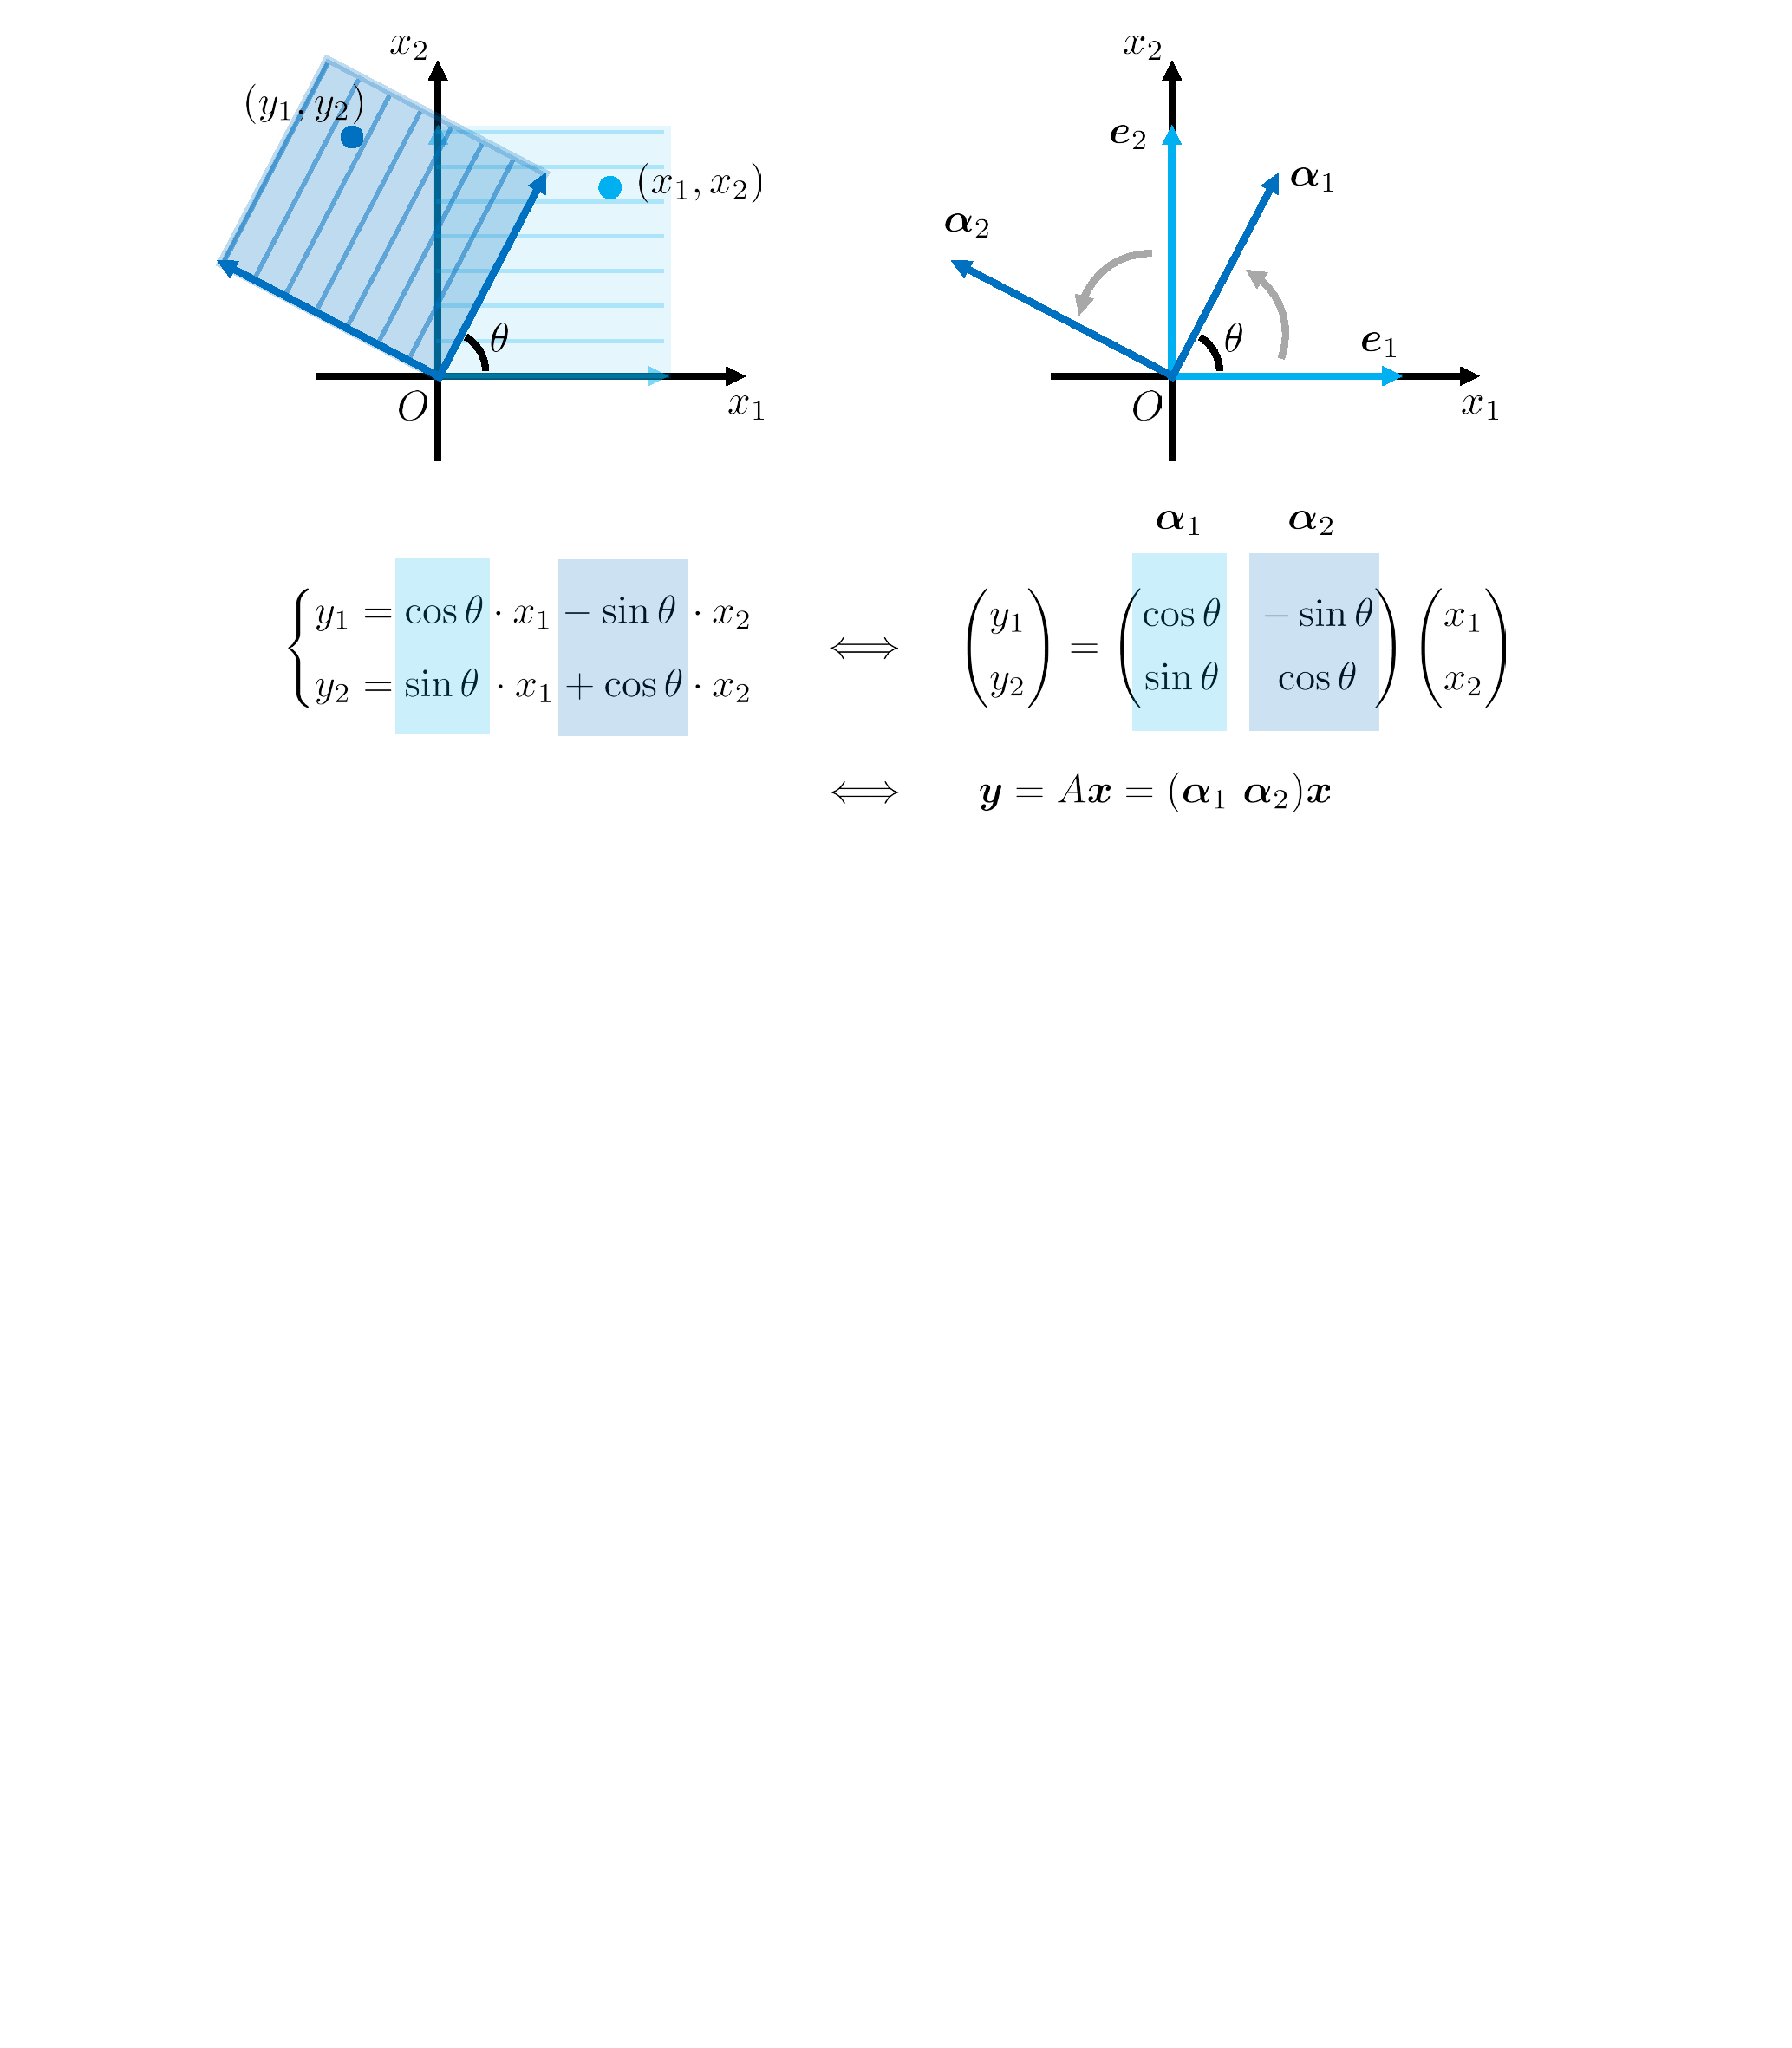
\includegraphics[trim=0 25cm 0 0, clip, width=1\textwidth]{fig/fig_bases.pdf}
    \caption{$\mathbb{R}^2$上旋转变换的矩阵}
    \label{fig:bases}
\end{figure}    

从这个想法也看出“基”在线性空间中的重要地位：
\textbf{一个线性映射被它作用在一组基上的像所唯一确定.}
刚刚我们在$\mathbb{K}^n \to \mathbb{K}^m$的线性映射中认识了这一点.
而因为任意$n$维线性空间$V$都和$\mathbb{K}^n$“没区别”，
这一点对于任意线性空间之间的线性映射都适用.
我们就依据这个原理写出任意线性映射的表示矩阵.

设$V$与$W$分别是数域$\mathbb{K}$上的$n$维与$m$维线性空间.
$\{ \bm{e}_1 , \bm{e}_2 , \cdots , \bm{e}_n \}$是$V$的一组基.
$\{ \bm{f}_1 , \bm{f}_2 , \cdots , \bm{f}_m \}$是$W$的一组基.
$V$和$W$的中的向量可以在各自的基下写出坐标来.
设$V$中向量$\bm{x}$在$\{\bm{e}_i\}$下的坐标是$(x_1 , x_2 , \cdots , x_n)$.
现在设$\mathcal{A}: V \to W$是线性映射，
且已知$V$的基向量在$\mathcal{A}$下的像$\mathcal{A}(\bm{e}_i)$.
如何用矩阵形式求出$\bm{y} = \mathcal{A}(\bm{x})$在$W$的基$\bm{f}_i$下的坐标$(y_1 , y_2 , \cdots , y_m)$？
我们只需要写出每个$\mathcal{A}(\bm{e}_i)$在$W$的基$\bm{f}_i$下的坐标：
\begin{eq1}
    \mathcal{A}(\bm{e}_i) &= a_{11} \bm{f}_1 + a_{21} \bm{f}_2 + \cdots + a_{m1}\bm{f}_m \mapsto (a_{11}, a_{21}, \cdots , a_{m1}) \\[4pt]
    \mathcal{A}(\bm{e}_2) &= a_{12} \bm{f}_1 + a_{22} \bm{f}_2 + \cdots + a_{m2}\bm{f}_m \mapsto (a_{12}, a_{22}, \cdots , a_{m2}) \\[4pt]
    \cdots \\[4pt]
    \mathcal{A}(\bm{e}_n) &= a_{1n} \bm{f}_1 + a_{2n} \bm{f}_2 + \cdots + a_{mn}\bm{f}_m \mapsto (a_{1n}, a_{2n}, \cdots , a_{mn}) \end{eq1}

将这些坐标以列向量的形式依次排列拼成一个矩阵：
\begin{eq1}
    A_{m \times n}= 
    \begin{pmatrix}
        a_{11} & a_{12} & \cdots & a_{1n} \\[2pt]
        a_{21} & a_{22} & \cdots & a_{2n} \\[2pt]
        \vdots & \vdots & \ddots & \vdots \\[2pt]
        a_{m1} & a_{m2} & \cdots & a_{mn}
    \end{pmatrix}\end{eq1}

这就是线性映射$\mathcal{A}$在\textbf{基$\{ \bm{e}_i \}$和基$\{ \bm{f}_i \}$下的表示矩阵.}
它的作用是把$\bm{x} \in V$在基$\{ \bm{e}_i \}$下的坐标$(x_1 , x_2 , \cdots , x_n)$
映为$\bm{y} = \mathcal{A} (\bm{x})$在基$\{ \bm{f}_i \}$下的坐标$(y_1 , y_2 , \cdots , y_m)$，
映射规则以矩阵乘法的形式给出：
\begin{eq1}
    \begin{pmatrix}
        y_1 \\[2pt] y_2 \\[2pt] \vdots \\[2pt] y_m
    \end{pmatrix}
    =
    \begin{pmatrix}
        a_{11} & a_{12} & \cdots & a_{1n} \\[2pt]
        a_{21} & a_{22} & \cdots & a_{2n} \\[2pt]
        \vdots & \vdots & \ddots & \vdots \\[2pt]
        a_{m1} & a_{m2} & \cdots & a_{mn}
    \end{pmatrix}
    \begin{pmatrix}
        x_1 \\[2pt] x_2 \\[2pt] x_3 \\[2pt] \vdots \\[2pt] x_n
    \end{pmatrix} \end{eq1}

特别需要注意的是，
用矩阵表示线性映射时，
必须说出选取的是$V$和$W$的哪一组基.
选取的基不同，
表示矩阵也会不同.
这个道理和向量的坐标表示一样.
因此，
可以把矩阵看作是线性映射的“坐标”.
这个观念与在$\mathbb{K}^n$中有所不同.
原来我们认为，“矩阵就是线性映射”.
现在我们认为，
\textbf{矩阵是线性映射在给定基下的表示.}
因此，
今后在一般的线性空间中，
我们必须开始严格区分“线性映射”与“矩阵”的概念，
正如我们必须区分“向量”与“坐标”的概念一样.

对于向量，
我们有任意$n$维线性空间$V$同构于$\mathbb{K}^n$的结论，
即坐标的线性运算可以代表向量的线性运算.
线性映射和矩阵之间也有类似的关系.

设$V$是$n$维线性空间，$W$是$m$维线性空间，
记$\mathrm{Hom}(V,W)$是全体$V \to W$的线性映射的集合，
记数域$\mathbb{K}$上全体$m \times n$矩阵的集合是$M_{m \times n}(\mathbb{K})$.
可以证明二者皆为数域$\mathbb{K}$上的$mn$维线性空间，
因此二者作为线性空间是同构的.
此外，线性映射有复合运算，
矩阵有乘法运算，
二者的乘法结构是一致的.
即：
\textbf{两个线性映射的复合的表示矩阵，
就是两个线性映射的表示矩阵的乘积.}
因此，
我们完全可以用矩阵的加法、数乘和乘法运算
来代表线性映射的加法、数乘和复合运算.



\subsubsection{线性变换与坐标变换}

设$V$是数域$\mathbb{K}$上的$n$维线性空间.
$\mathcal{A}$是其上的线性变换.
既然是在同一个空间，
对于映射前后的向量$\bm{x}$与$\bm{y} =\mathcal{A} (\bm{x})$，
完全可以选择同一组基$\{ \bm{e}_1 , \bm{e}_2 , \cdots , \bm{e}_n \}$来写出它们的坐标
（分别记为$\bm{X}$和$\bm{Y}$），
不用自找麻烦地选择两组不同的基.
此时可以写出$\mathcal{A}$在这组基下的表示矩阵及坐标映射规则：
\begin{eq1}
    \begin{pmatrix}
        y_1 \\[2pt] y_2 \\[2pt] \vdots \\[2pt] y_n
    \end{pmatrix}
    =
    \begin{pmatrix}
        a_{11} & a_{12} & \cdots & a_{1n} \\[2pt]
        a_{21} & a_{22} & \cdots & a_{2n} \\[2pt]
        \vdots & \vdots & \ddots & \vdots \\[2pt]
        a_{n1} & a_{n2} & \cdots & a_{nn}
    \end{pmatrix}
    \begin{pmatrix}
        x_1 \\[2pt] x_2 \\[2pt] \vdots \\[2pt] x_n
    \end{pmatrix} 
    ~~~
    \Longleftrightarrow
    ~~~
    \bm{Y} = A \bm{X} \end{eq1}

可以看到表示矩阵$A$是$n$阶方阵.
它的第$i$个列向量就是$\mathcal{A} (\bm{e}_i)$在基$\{ \bm{e}_1 , \bm{e}_2 , \cdots , \bm{e}_n \}$下的坐标.

目前为止，
我们一直在讨论线性映射：
$V$中的向量$\bm{x}$被变换成了另一个向量$\bm{y}$.
在同一组基下，
变换前后的向量坐标不同，
变换的规则由矩阵方程$\bm{Y} = A \bm{X}$描述.
然而也可以用一种截然不同的角度理解这个方程：
$\bm{X}$和$\bm{Y}$是同一个向量在两组不同的基下的坐标，
$\bm{Y} = A \bm{X}$描述的是基变换下同一个向量坐标的变换规则.
简而言之，
\textbf{线性变换}说的是\textbf{基不变，向量在变}，
而\textbf{坐标变换}说的是\textbf{向量不变，基在变}.

为什么同一条公式能引入两种不同的理解？
我们以旋转变换为例说明.
在图\ref{fig:rotcoord}中，
左侧展示的是$\mathbb{R}^2$上逆时针旋转$\theta$角的线性变换.
以$\{ \bm{e}_1 , \bm{e}_2\}$为基，
浅蓝色点所代表的向量$\bm{x}$坐标是$\bm{X} = (x_1,x_2)^T$，
它在被旋转之后变成了另一个向量$\bm{y}$，
其坐标为$\bm{Y} = (y_1,y_2)^T$.
而右图则展示了一个相反的操作：
把浅蓝色点所代表的向量固定不动，
而把基$\{ \bm{e}_i \}$顺时针旋转$\theta$角，
变成了一组新基$\{ \bm{f}_i \}$.
在这组新的基下，
同一个向量又获得了新坐标$\bm{Y} = (y_1,y_2)^T$.

\begin{figure}[H] 
    \centering
    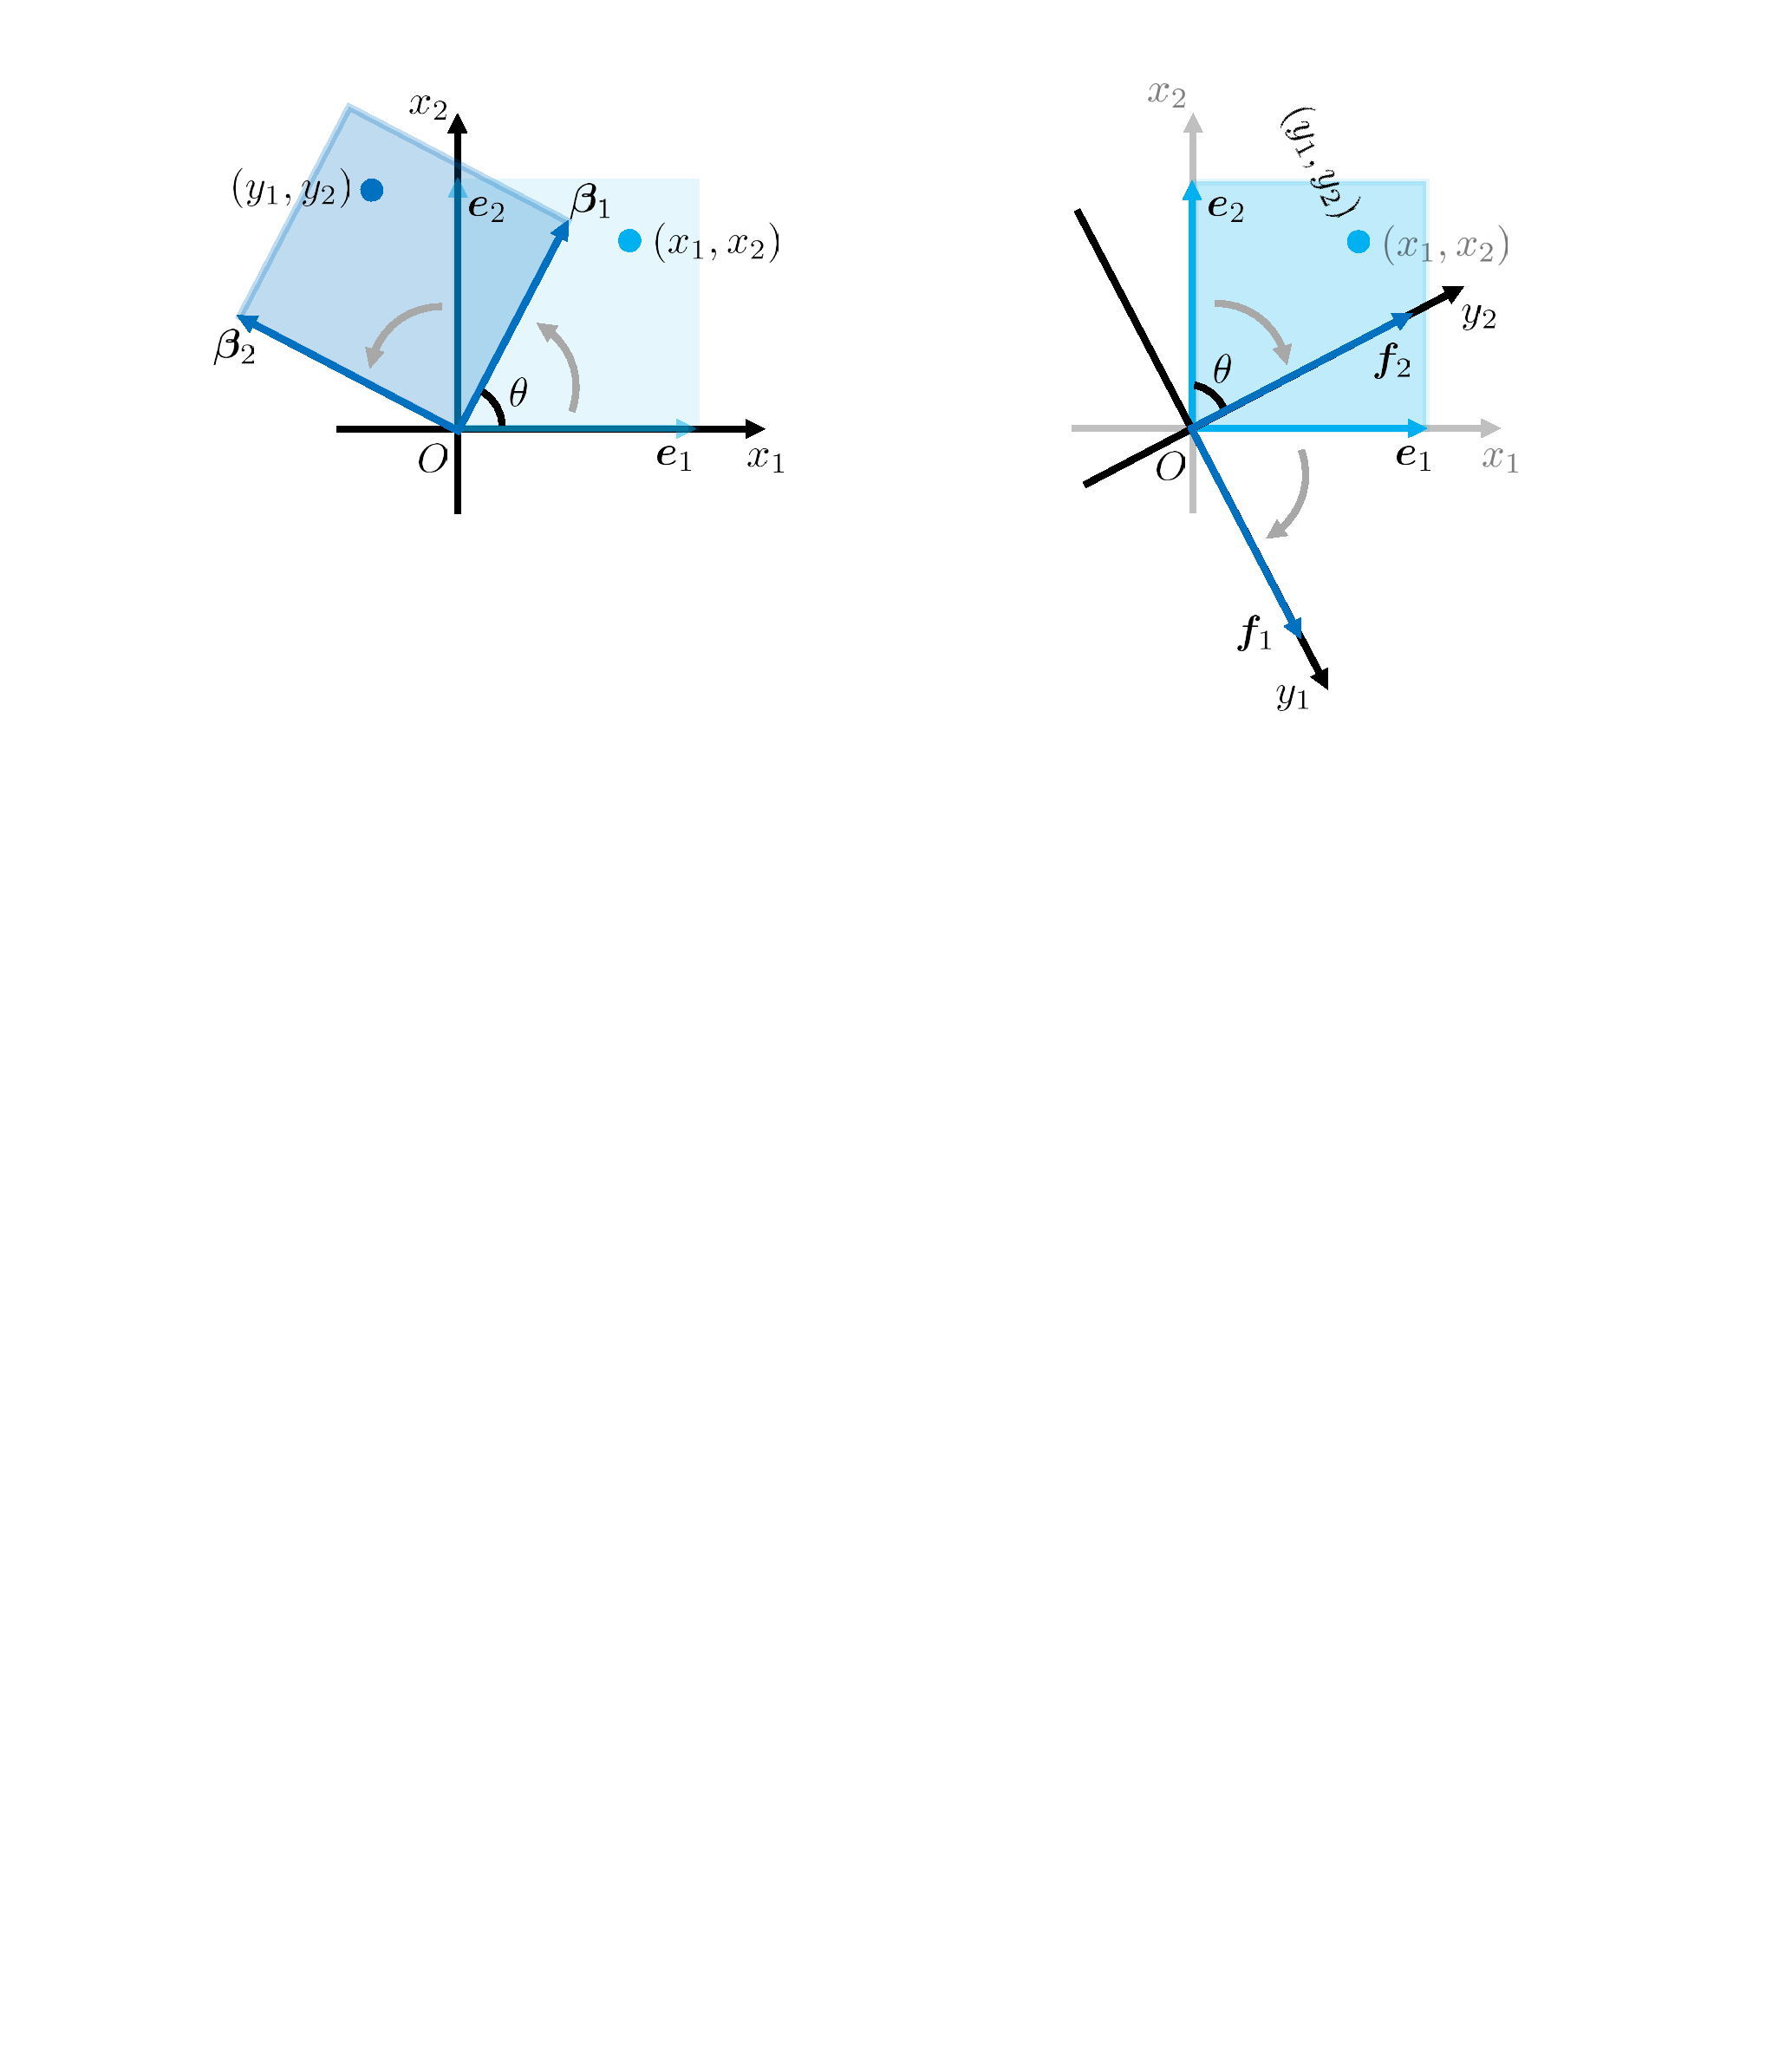
\includegraphics[trim=0 26cm 0 0, clip, width=1\textwidth]{fig/fig_rotcoord.pdf}
    \caption{向量旋转vs坐标系旋转}
    \label{fig:rotcoord}
\end{figure}    

“向量逆时针旋转$\theta$角”与
“坐标系（基）顺时针旋转$\theta$角”这两件事真的有任何区别吗？
细想之下，
图\ref{fig:rotcoord}中$x_1$与$x_2$坐标轴虽然看似总是固定不动，
但只是我们以纸面（或者电子屏幕）为参照物的错觉.
在我们讨论问题的过程中，
并未引入第三个坐标系或参考物，
那么我们实际上无从判断$x_1$与$x_2$坐标轴的“方向”究竟是变了还是没变.
因此，“向量逆时针旋转$\theta$角”与
“坐标系（基）顺时针旋转$\theta$角”只是对同一个相对运动现象的两种不同描述.

借助这个例子，
我们很直观地看到：
\textbf{对一个向量施加线性变换$\mathcal{A}$的效果，
与对一组基施加一个逆向的线性变换$\mathcal{A}^{-1}$的效果是等同的}.
这是一个相当自然的原理，
因此这里省去篇幅不再解释如何证明它.
我们只解释如何更严肃地用数学语言描述线性变换与坐标变换的关系.
设$V$中的一组基$\{ \bm{e}_i \}$变换成$\{ \bm{f}_i \}$.
别忘了，
一组基在映射下的像可以唯一确定一个线性映射$\mathcal{B}$.
我们写出$\mathcal{B}$在基$\{ \bm{e}_i \}$下的表示矩阵.
先写出$\{ \bm{f}_i \}$在基$\{ \bm{e}_i \}$下的展开以及坐标：
\begin{eq1}
    \bm{f}_1 = \mathcal{B}(\bm{e}_i) &= a_{11} \bm{e}_1 + a_{21} \bm{e}_2 + \cdots + a_{n1}\bm{e}_n \mapsto (a_{11}, a_{21}, \cdots , a_{n1}) \\[4pt]
    \bm{f}_2 = \mathcal{B}(\bm{e}_2) &= a_{12} \bm{e}_1 + a_{22} \bm{e}_2 + \cdots + a_{n2}\bm{e}_n \mapsto (a_{12}, a_{22}, \cdots , a_{n2}) \\[4pt]
    \cdots \\[4pt]
    \bm{f}_n = \mathcal{B}(\bm{e}_n) &= a_{1n} \bm{e}_1 + a_{2n} \bm{e}_2 + \cdots + a_{nn}\bm{e}_n \mapsto (a_{1n}, a_{2n}, \cdots , a_{nn}) \end{eq1}

将这些坐标以列向量的形式依次排列拼成一个矩阵，
就得到$\mathcal{B}$在基$\{ \bm{e}_i\}$下的表示矩阵：
\begin{eq1}
    A = 
    \begin{pmatrix}
        a_{11} & a_{12} & \cdots & a_{1n} \\[2pt]
        a_{21} & a_{22} & \cdots & a_{2n} \\[2pt]
        \vdots & \vdots & \ddots & \vdots \\[2pt]
        a_{n1} & a_{n2} & \cdots & a_{nn}
    \end{pmatrix}\end{eq1} 

请注意，
因为$\{ \bm{e}_i \}$的像$\{ \bm{f}_i \}$是$V$的一组基，
是一个线性无关的向量组，
因此$\mathcal{B}$在基$\bm{e}_i$下的表示矩阵是列满秩的，
即：\textbf{基变换$\mathcal{B}$一定是可逆变换，即$V$的一个自同构，
其表示矩阵是可逆矩阵.}
在教材中，往往会引进一种形式写法来表示基变换：
\begin{eq1}
    (\bm{f}_1 , \bm{f}_2 , \cdots , \bm{f}_n)
    = 
    (\bm{e}_1 , \bm{e}_2 , \cdots , \bm{e}_n)
    \begin{pmatrix}
        a_{11} & a_{12} & \cdots & a_{1n} \\[2pt]
        a_{21} & a_{22} & \cdots & a_{2n} \\[2pt]
        \vdots & \vdots & \ddots & \vdots \\[2pt]
        a_{n1} & a_{n2} & \cdots & a_{nn}
    \end{pmatrix} \end{eq1}

其中的“行向量”是由$V$的一组基而非数域$\mathbb{K}$的元素构成，
只是在形式上用矩阵方程表示它们之间的关系.
在这种写法下，
等式右侧的$n$阶方阵与之前给出的$\mathcal{B}$的表示矩阵是一样的.
这个矩阵称为从$\{\bm{e}_i \}$到$ \{ \bm{f}_i \}$的\textbf{过渡矩阵}.
而基的线性变换引起了一个坐标变换$\bm{Y} = A \bm{X}$.
这里的坐标变换矩阵$A$即是过渡矩阵之逆.




\subsubsection{*主动观点与被动观点}

对于同一个矩阵方程$\bm{Y} = A \bm{X}$，
现在有了两种不同的理解：\medskip

(1)~~\textbf{主动观点}：坐标系没动，向量按照矩阵$A$变换，连同着它的坐标从$\bm{X}$变成了$\bm{Y}$.

(2)~~\textbf{被动观点}：向量没动，基按照矩阵$A^{-1}$变换，引起向量的坐标从$\bm{X}$变换成$\bm{Y}$.\medskip

正如本节一开始所讨论的，
这两种观点等价性很明显，
甚至是不言而喻的.
但其中的意义却很深刻，
可以帮助我们理解许多有趣的问题.


为了提高被动观点的可视化程度，
我们可以通过灰色的坐标网格线来展示坐标系的变化.
坐标网格以平行等距的形式绘制.
根据线性变换的要求，
当坐标系变换时，
新的坐标网格仍然是平行等距的.
我们也能轻易地通过旧的和新的坐标网格分别读出变换前后向量的坐标.
为了体现这样做的用处，
图\ref{fig:ruler}展示了一个相对“没什么特点”的线性变换.
注意$(x',t')$在左侧图和右侧图中与坐标网格的相对位置是相同的
（横纵都是大约$2$格多一点），
这是主动观点与被动观点等价性的一种直观体现.


\begin{figure}[H] 
    \centering
    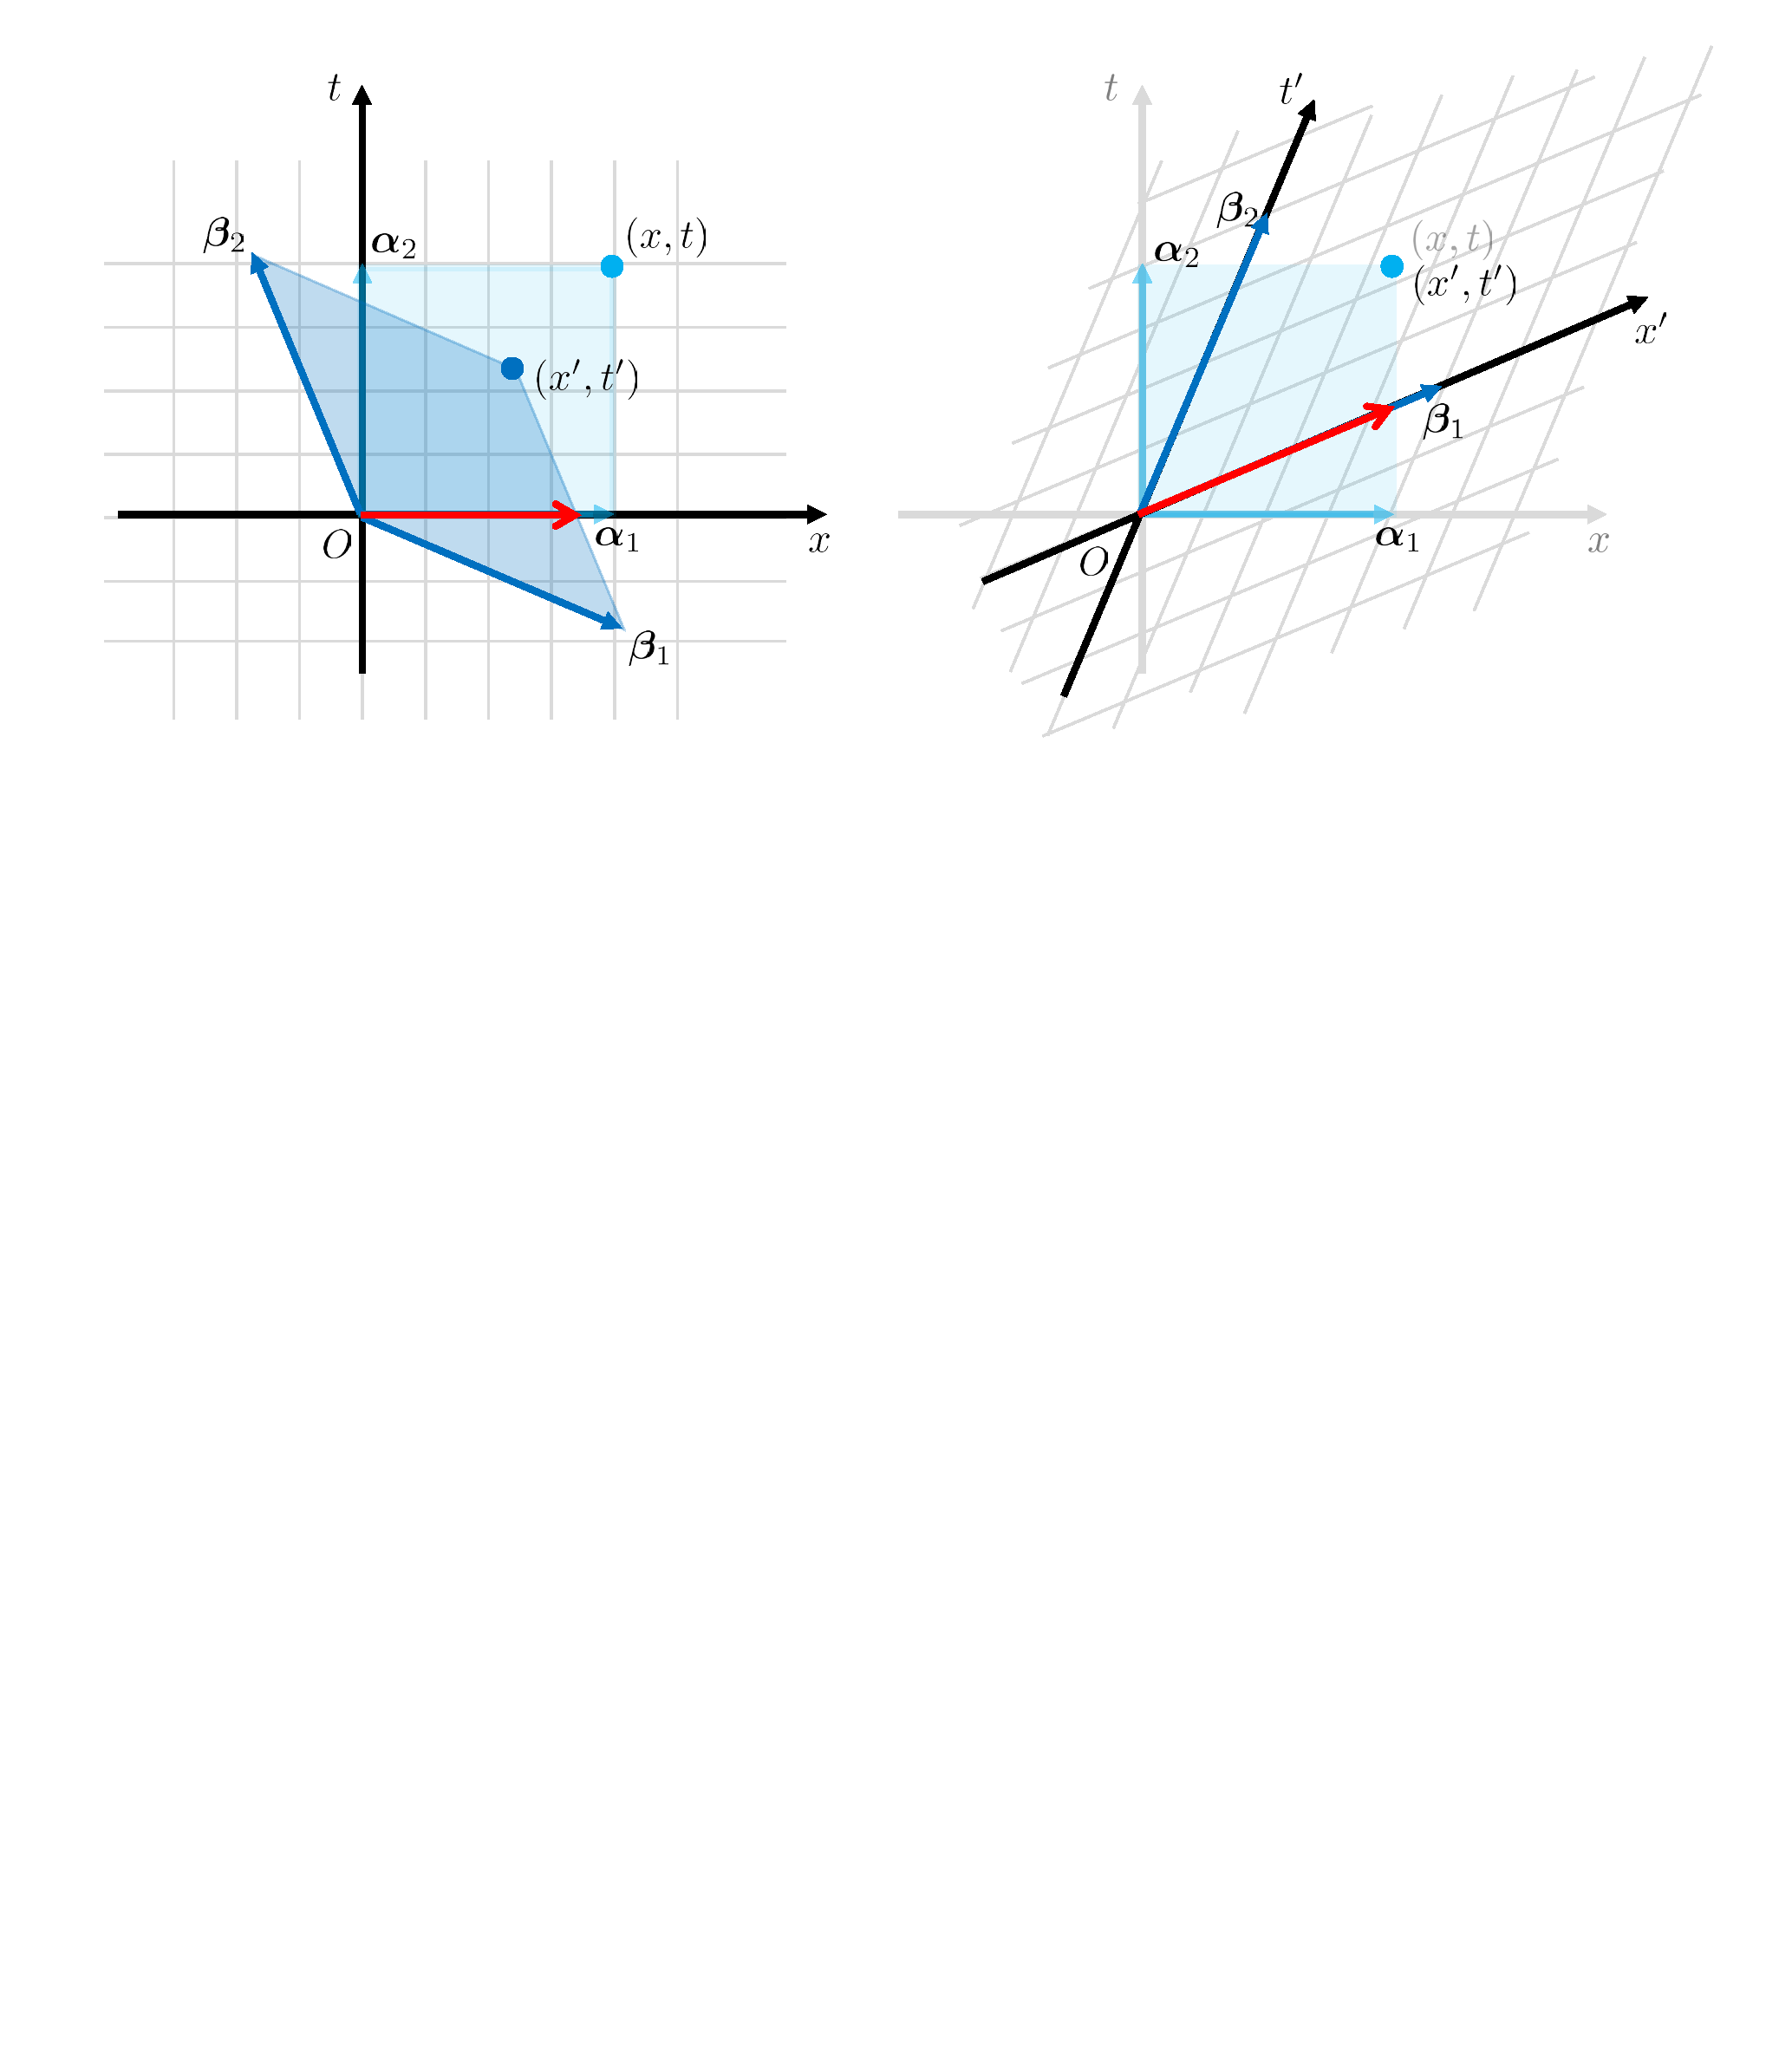
\includegraphics[trim=0 25cm 0 0, clip, width=1\textwidth]{fig/fig_ruler.pdf}
    \caption{洛伦兹变换的主动观点与被动观点. 
    左图显示了主动观点的图像，向量$\bm{\alpha}_1$是一把单位长度的“尺子”.
    浅蓝色区域是尺子静止的时空图，
    蓝色区域是尺子匀速运动的时空图.
    在$t=0$时刻测量动尺的长度，
    结果如红色箭头所示，
    是比单位长度$\bm{\alpha}_1$要短的.
    右图显示了被动观点的图像.
    尺子的时空图在不同参考系下均为浅蓝色区域.
    在相对于尺子运动的参考系（旁观者）中，
    在$t'=0$时刻测量尺子的长度，
    结果如红色箭头所示，
    是比$x'-t'$系中的单位长度$\bm{\beta}_1$要短的.
    注意在$x-t$中，
    红色箭头的两端不是同时的（即$t$坐标不同）.
    }
    \label{fig:ruler}
\end{figure}

主动观点和被动观点在原则上没有优劣之分，
但是在观察世界时，
我们作为观测者容易偏执一端，
只采取我们习惯的观点，
而忽略另一种可能更具实际价值的观点.
打个比方来说，
当我们抬头望天时，
直觉上会认为是太阳围绕着在地球转动，
这是以“静止”的地面为参考系观测得出的结论.
但实际上，
“太阳不动而地球自转”可能是更恰当的观点.
今天我们之所以能轻松地评述这两种观点，
是因为我们的眼界能跳出地球，甚至跳出太阳系，
从旁观者的角度观察自己的处境.
但是作为当局者时，
我们经常无法想到可以转换视角来看问题.

图\ref{fig:ruler}展示的线性变换是洛伦兹于1904年发表的\textbf{洛伦兹变换}.
这是爱因斯坦的狭义相对论中描述不同参考系下时空变换规律的公式：
\begin{eq1}
    \begin{pmatrix}
        x' \\[2pt] t'    
    \end{pmatrix}
    =
    \begin{pmatrix}
        \gamma  & -\gamma \beta \\[2pt]
        -\gamma \beta & \gamma
    \end{pmatrix}
    \begin{pmatrix}
        x \\[2pt] t
    \end{pmatrix} 
    ,
    ~~~\text{其中}~
    \beta = \frac{v}{c},~ \gamma = \frac{1}{\sqrt{1-\beta^2}}
    \end{eq1}

在狭义相对论之前，
物理学界的主流观点认为光波传播需要一种名为“以太”的介质，
并假设它是绝对静止的参考系.
1887年，
迈克尔逊-莫雷实验未能探测到地球相对于以太的运动，
几乎完全推翻了以太假说，
物理学界陷入一片迷雾.
由于绝对时空观在人们心中根深蒂固，
许多物理学家仍不愿放弃以太这种绝对时空的载体，
希望修补以太理论.
洛伦兹就是其中之一.
他认为，
物体在以太中运动时，
物体在运动方向上会被“缩短”.
这可以从洛伦兹变换的\textbf{主动观点}出发推导出来（图\ref{fig:ruler}左）.
之所以说是主动观点，
是因为洛伦兹变换虽然涉及空间坐标$x$和时间坐标$t$的共同变换，
但洛伦兹只将它视为辅助的数学技巧，
并不蕴含真实的物理.
真正的物理过程在于物体的分子间作用力会与以太发生某种作用，
使得物体发生物理上“真实”的缩短.

在狭义相对论框架下，
洛伦兹变换仍然是正确的公式.
著名的“动尺缩短效应”
与洛伦兹的预测在数学上同根同源.
然而，
狭义相对论对于洛伦兹变换的解读颠覆性地采用\textbf{被动观点}.
在对于“动尺缩短效应”的分析中，
运动的物体本身并没有发生真实的变化，
只不过参考系的相对运动会引起时空的变换，
同一个物体在不同的参考系中“测量标准”不同，
当然会测出不同的长度
（例如，在“动尺”参考系中同时测量尺子的两端，
在旁观者眼中就不是同时的）
（图\ref{fig:ruler}右）.

在这个例子中，
主动观点与被动观点的区别折射出人们对于“时空”认知的根本性区别.
即便对于今人，
要摈弃绝对时空观，
接受“时空会变”的被动观点，
仍然极富挑战性.

\subsection{线性映射的分解}

\subsubsection{矩阵的等价和相似}

设$n$维线性空间$V$有一组基$\{ \bm{e}_i \}$，
$m$维线性空间$W$有一组基$\{ \bm{f}_i \}$.
线性映射$\mathcal{A}: V \to W$在基$\{ \bm{e}_i \}$和
$\{ \bm{f}_i \}$下的表示矩阵为$A_{m \times n}$.
$\bm{y} = \mathcal{A} (\bm{x})$的坐标由$\bm{Y} = A \bm{X}$给出.
现在，
如果两个空间中各自发生基变换
$\{ \bm{e}_i \} \mapsto \{ \bm{e}'_i \}$和
$\{ \bm{f}_i \} \mapsto \{ \bm{f}'_i \}$，
分别以$P_{n \times n}$和$Q_{m \times m}$为过渡矩阵，
那么$\mathcal{A}$的表示矩阵会怎么变化？
设$\bm{x}$和$\bm{y}$在各自的新基$\{ \bm{e}'_i \}$和$\{ \bm{f}'_i \}$下的坐标分别为$\bm{X}'$和$\bm{Y}'$.
则$P\bm{X}' = \bm{X}, ~Q\bm{Y}' = \bm{Y}$.
于是有：
\begin{eq1}
    Q \bm{Y}' = A P \bm{X}', ~~
    \text{即}~  \bm{Y}' = Q^{-1}AP \bm{X}'
\end{eq1}

可见，
线性映射$\varphi$在新基下的表示矩阵为$Q^{-1}AP$.
也就是说，
如果存在$n$阶可逆矩阵$P_1$和$m$阶可逆矩阵$P_2$，
使得$B = P_2 A P_1$，
则矩阵$A_{m \times n}$和$B_{m \times n}$是\textbf{同一个线性映射在不同基下的表示矩阵.}
这恰好是讲义第二章中提及的\textbf{矩阵等价}的概念.
当时我们分析过，
两个$m \times n$矩阵等价当且仅当它们的秩相等.
于是现在我们知道，
\textbf{所有秩相等的$m \times n$的矩阵都可以表示同一个线性映射.}
同时也知道，
秩虽然是在矩阵中定义的，
却可以作为线性映射的属性来看待，
即与基的选择无关的一个性质.
其中的根本原因在于，
秩其实是线性映射像空间的维数，
后者自然是与基的选择无关的.

在上面的讨论中，
我们总是在讨论同一个线性映射$\mathcal{A}$，
由于基的变换导致它的表示矩阵发生变换.
这是一种\textbf{被动观点}.
我们现在再从\textbf{主动观点}来描述矩阵的等价，
即：取定每个空间的基不变，等价变换下不同的矩阵代表了不同的线性映射.
这里，我们把$P_1$和$P_2$看成两个同构映射的表示矩阵.
设$V_1$和$W_1$分别是$n$维和$m$维线性空间，
$P_1$是同构映射$\sigma_1 : V_1 \to V$的表示矩阵，
$P_2$是同构映射$\sigma_2 : W \to W_1$的表示矩阵.
则等价变换后的矩阵$B = P_2 A P_1$表示了一个复合的线性映射$\sigma_2 \circ \mathcal{A} \circ \sigma_1$，
它是$ V_1 \to W_1$的线性映射.
照这种看法，
请问$A$与$B$所代表的线性映射$\mathcal{A}$与$\sigma_2 \circ \mathcal{A} \circ \sigma_1$之间有何区别？
答案是\textbf{本质上没有区别}.
在同构的意义下，
$V_1$与$V$，
$W_1$与$W$本就无从区分，
同构映射$\sigma_1$和$\sigma_2$的作用只是方便我们在两个“无从区分”的空间之间进行转换而已.
因此，
矩阵等价在主动观点下的意义是告诉我们：
\textbf{在线性空间同构的意义下，所有秩相等的线性映射本质上没有区别.}
\medskip

上面的这些结论的意义是深刻的，
但用途也有限.
我们研究线性映射，
当然不是光研究秩就满足了.
然而对于矩阵等价而言，
同一个线性映射的不同表示矩阵（或不同的线性映射）
在秩以外的区别是“看不清楚”的.
从被动观点来讲，
这是因为我们允许$V$和$W$的基各自做任意的变换，
这自由度太高了.

本课程的一个重点是研究线性变换的表示矩阵.
对于$n$维空间上的线性变换$\mathcal{A} : V \to V$，
根据上一节的介绍，
只需选定一组基$\{ \bm{e}_i \}$就能写出其表示矩阵$A$.
若基变换$\{ \bm{e}_i \} \mapsto \{ \bm{e}'_i \}$
以$P_{n \times n}$为过渡矩阵，
新旧坐标之间的关系
$P\bm{X}' = \bm{X}, ~ P\bm{Y}' = \bm{Y}$.
于是有：
\begin{eq1}
    P \bm{Y}' = A P \bm{X}', ~~
    \text{即}~  \bm{Y}' = P^{-1}AP \bm{X}'
\end{eq1}

可见，
线性变换$\mathcal{A}$在新基下的表示矩阵为$P^{-1}AP$.
也就是说，
如果存在$n$阶可逆矩阵$P$使得
$B = P^{-1}AP$，
则矩阵$A$和$B$是
\textbf{同一个线性变换在不同基下的表示矩阵}.
此时我们称矩阵$A$和$B$是\textbf{相似}的，
记作$A \sim B$.
变换$A \mapsto P^{-1}AP$称为\textbf{相似变换}.
可以证明相似变换是一种等价关系：

\medskip




(1)~~反身性：取$P = I$，显然$I^{-1} A I = A$，
因此$A \sim A$.

(2)~~对称性：如果$A \sim B$，
即存在可逆矩阵$P$使得$B = P^{-1}AP$.
取$Q = P^{-1}$，则$A = Q^{-1}BQ$，
因此$B \sim A$.

(3)~~传递性：
如果$A \sim B , ~B \sim C$，
即存在可逆矩阵$P,Q$，
使得$B = P^{-1} A P, ~C = Q^{-1} B Q$，
则$C = Q^{-1} P^{-1} A PQ$.
取$R = PQ$，
则$C = R^{-1} A R$，
即$A \sim C$.
\medskip

矩阵在相似关系下的不变量称为\textbf{相似不变量}.
一个线性映射虽然可以有众多表示矩阵，
但是这些表示矩阵应该有共同的，
与基的选择无关的性质.
表示矩阵的这类性质可以看成是线性映射本身的属性，
这就是相似不变量的意义.
显然，
矩阵相似是矩阵等价的一种特殊情况，
所以\textbf{矩阵的秩是相似不变量}.
另外，
利用行列式的性质容易证明，
\textbf{矩阵的行列式也是相似不变量.}
其背后的含义是，
\textbf{线性映射对体积的缩放比例是线性映射的一个属性，
与基的选择无关.}
因此，
我们完全可以越过矩阵，
直接谈论线性映射的秩$\mathrm{rank}(\mathcal{A})$
和线性变换的行列式$\det \mathcal{A}$.
$\det \mathcal{A}$这种记法是有一定实用性的，
但实际一般不采用$\mathrm{rank}(\mathcal{A})$这种记法，
因为$\dim \operatorname{Im} \mathcal{A}$显得意思更加明确.
在讲义第六章中，
将对相似不变量进行更深入的讨论.

根据“相似关系是等价关系”的思想，
我们希望给出相似关系的完全不变量，
或者以某种算法找到每个相似类的代表元，
从而完成对矩阵作为线性映射表示矩阵的分类工作.
所谓找“代表元”，
是希望对于任意给定的$n$阶方阵，
都能找到一个与之相似且形式尽量简单的方阵.
换句话说，
\textbf{对于$n$维线性空间$V$上任意给定的线性变换$\mathcal{A}$，
去找$V$上的一组基，
使得$\mathcal{A}$在这组基下的表示矩阵尽量简单.}
上述那种“最简单”的表示矩阵称为\textbf{相似标准型}.

什么样的矩阵算是“最简单”的矩阵？
最容易想到的是对角矩阵.
可惜事实上，
并非所有方阵都一定相似于某个对角矩阵.
这样的话，
该选择什么类型的矩阵作为相似标准型，
又该如何计算一个任意矩阵的相似标准型？
这提出了一个较大的课题.
在线性代数课程中，
我们只会解决这个课题的一小部分.

（注：为了方便，
我们将一直采用被动观点处理矩阵的相似.
当然，
用主动观点来理解也是可行，而且完全等价的.）
\medskip

考察以下两个$4$阶方阵：
\begin{eq1}
    A = 
    \begin{pmatrix}
        0 & \sqrt{2} & 0 & -\sqrt{2} \\[8pt]
        \frac{\sqrt{2}}{2} & -\sqrt{2} & -\frac{\sqrt{2}}{2} & \sqrt{2} \\[8pt]
         0 & 2\sqrt{2} & \sqrt{2} & -\sqrt{2} \\[8pt]
         \sqrt{2} & -2\sqrt{2} & -\frac{\sqrt{2}}{2} & 2\sqrt{2}
    \end{pmatrix}
    ~~~~~
    B = 
    \begin{pmatrix}
        \frac{\sqrt{2}}{2} & -\frac{\sqrt{2}}{2} & 0 & 0 \\[8pt]
        \frac{\sqrt{2}}{2} & \frac{\sqrt{2}}{2} & 0 & 0 \\[8pt]
         0 & 0 & \frac{\sqrt{2}}{2} & \frac{\sqrt{2}}{2} \\[8pt]
         0 & 0 & -\frac{\sqrt{2}}{2} & \frac{\sqrt{2}}{2} 
    \end{pmatrix}\end{eq1}

取过渡矩阵$P$：
\begin{eq1}
    P
    = 
    \begin{pmatrix}
        1 & 1 & 0 & 0 \\[4pt]
        0 & 1 & 1 & 0 \\[4pt]
        0 & 0 & 1 & 1 \\[4pt]
        2 & 0 & 0 & 1 
    \end{pmatrix}\end{eq1}

可以验证：
\begin{eq1}
    A = P^{-1} B P  \end{eq1}
即矩阵$A$与$B$相似，
它们是同一个线性映射$\varphi$在不同基下的表示矩阵.

观察表示矩阵$A$，
很难看出个所以然来：
$A$的矩阵元很杂乱，
而且$4$维空间的几何图像本来就无法想象.
然而，
$B$作为一个\textbf{分块对角矩阵}却容易理解得多.
设被$\varphi$变换前后（与$B$相同的基下）的向量坐标为$\bm{X} = (x_1, x_2, x_3, x_4)^T$
和$\bm{Y} = (y_1, y_2, y_3, y_4)^T$.
根据矩阵乘法的规则，
$\bm{Y} = B \bm{X}$的表达式可以写为以下两部分：
\begin{eq1}
    \begin{pmatrix}
        y_1 \\[12pt]
        y_2 
    \end{pmatrix}
    =
    \begin{pmatrix}
        \frac{\sqrt{2}}{2} & -\frac{\sqrt{2}}{2}\\[8pt]
        \frac{\sqrt{2}}{2} & \frac{\sqrt{2}}{2}
    \end{pmatrix}
    \begin{pmatrix}
        x_1 \\[12pt]
        x_2 
    \end{pmatrix},
    ~~~~~
    \begin{pmatrix}
        y_3 \\[12pt]
        y_4 
    \end{pmatrix}
    =
    \begin{pmatrix}
        \frac{\sqrt{2}}{2} & \frac{\sqrt{2}}{2}\\[8pt]
        -\frac{\sqrt{2}}{2} & \frac{\sqrt{2}}{2}
    \end{pmatrix}
    \begin{pmatrix}
        x_3 \\[12pt]
        x_4 
    \end{pmatrix} \end{eq1}

这实际上是两个$2$维空间的旋转变换，
且这两个$2$阶方阵恰是原来$4$阶方阵的两个非零的\textbf{矩阵块}.
于是，$B$的作用被分解成两部分：
一是对$x_1 - x_2$平面施加了逆时针旋转$45°$的变换；
二是对$x_3 - x_4$平面施加了顺时针旋转$45°$的变换.
这样来看，
线性映射$\varphi$的作用方式一下子就清晰可见了.

从这个例子中可以看出，
\textbf{高维的线性变换可以分解到低维的线性子空间上}，
从而让线性变换的结构显得更简单易懂.
这种分解方式原则上只与线性变换在$V$上的作用方式有关，
与基的选取及表示矩阵的形式无关.
但是，如果把表示矩阵写成\textbf{分块对角矩阵}的形式，
则能让我们一眼看出线性变换的分解.
依据这种“分解”的思想，
我们希望用分块对角矩阵来构造相似标准型.
也就是说，
\textbf{计算相似标准型，实质就是搞清楚线性变换如何分解}.
本章的剩余部分就将落实这个思想.


\subsubsection{线性空间的直和分解}

我们首先需要说明的是，
对一个线性空间进行“分解”是什么意思.

设$n$维线性空间$V$有两个线性子空间$V_1$和$V_2$.
$V_1$与$V_2$的\textbf{和}定义为：
\begin{eq1}
    V_1 + V_2 = \{  \bm{\alpha}+\bm{\beta} ~|~ \bm{\alpha} \in V_1 , ~\bm{\beta} \in V_2 \} \end{eq1}

容易验证，
$V_1 + V_2$也是$V$的一个线性子空间
（见习题部分）.
我们自然会问，
$V_1 + V_2$的维数如何确定？
我们给出如下的维数公式：
\begin{eq1}
    \text{dim}~(V_1 + V_2) = \text{dim}~V_1 + \text{dim}V_2 - \text{dim}~(V_1 \cap V_2)\end{eq1}
这里，$V_1 \cap V_2$也是$V$的一个线性子空间.
该公式可以简单地用容斥原理来理解：
假设先取$V_1 \cap V_2$的一组基
$\{ \bm{\alpha}_1, \bm{\alpha}_2,\cdots ,  \bm{\alpha}_m \}$，
分别将其扩充成$V_1$的一组基$\{ \bm{\alpha}_1,\cdots ,  \bm{\alpha}_m ,  \bm{\alpha}_m+1 , \cdots , \bm{\alpha}_{n_1}\}$
和$V_2$的一组基$\{ \bm{\alpha}_1,\cdots ,  \bm{\alpha}_m ,  \bm{\beta}_{m+1} , \cdots , \bm{\beta}_{n_2}\}$.
这两组基的并集应是$V_1 + V_2$的一组基，
其向量个数为$n_1 + n_2 - m$（证明见教科书）.

如果$V$表示成两个线性子空间之和$V_1 + V_2$，
那么可以说这是对$V$的一个“分解”.
对此的一种理解方式是，
\textbf{线性空间的分解规定了向量的分解}.
因为根据定义，
$V=V_1 + V_2$意味着任取$\bm{v} \in V$，
都存在$\bm{v}_1 \in V_1 , ~\bm{v}_2 \in V_2$，
使得$\bm{v}$被分解成$\bm{v} = \bm{v}_1 + \bm{v}_2$.
但坏消息是，
这种向量分解的方式可能不是唯一的.
根本原因在于两个子空间的公共部分$V_1 \cap V_2$可以“任意调度”：
若取非零向量$\bm{w} \in V_1 \cap V_2$，
则$\bm{u}_1 = \bm{v}_1 + \bm{w} \in V_1 , ~\bm{u}_2 = \bm{v}_2 - \bm{w} \in V_2$，
则$\bm{v} = \bm{v}_1 + \bm{v}_2 = \bm{u}_1 + \bm{u}_2$就是两个不同的分解.
为了避免这种情况，
在谈论线性空间或向量的分解时，
我们会要求$V_1 \cap V_2$是平凡子空间$\{ \bm{0} \}$.
由此，引出了\textbf{直和}的概念.\medskip

\textbf{直和的定义}~~
\textit{设$V_1$和$V_2$是线性空间$V$的子空间.
若$V_1 \cap V_2 = \{ \bm{0} \}$，
则称$V_1 + V_2$为直和，记为：$V_1 \oplus V_2$.
}

\textit{该定义可以自然推广至任意有限个子空间之和： 
设$V_i~(i=1,2,\cdots, m)$是$V$的$m$个子空间.
若对一切$i$满足}
\begin{eq1}
    V_i \cap (V_1 +\cdots +  V_{i-1} + V_{i} + \cdots + V_m) = \{ \bm{0} \} \end{eq1}

\textit{则称$V_1 + V_2 + \cdots + V_m$为直和，记为：
$V_1 \oplus V_2 \oplus \cdots \oplus V_m$.}\medskip

如果$V = V_1 \oplus V_2 \oplus \cdots \oplus V_m$，
我们称$V_1 \oplus V_2 \oplus \cdots \oplus V_m$是对$V$的一个\textbf{直和分解}.
我们讨论线性空间的分解时，
默认是指直和分解.
直和分解意味着，
任取$\bm{v} \in V$，
都存在$\bm{v}_1 \in V_1 , ~\bm{v}_2 \in V_2, \cdots \bm{v}_m$，
使得$\bm{v}$被分解成$\bm{v} = \bm{v}_1 + \bm{v}_2+ \cdots + \bm{v}_m$，
且\textbf{这种分解方式是唯一的}.

一种特殊的直和分解是将$V$分解成$n$个$1$维子空间的直和：
$V = \langle \bm{e}_1 \rangle \oplus \langle \bm{e}_2 \rangle \oplus \cdots \oplus \langle \bm{e}_n \rangle$，
其中$\{ \bm{e}_1 , \bm{e}_2, \cdots , \bm{e}_n \}$是$V$的一组基.
则此时任意向量$\bm{v} \in V$的唯一分解就是按这组基展开.
这是一种最彻底的直和分解.
自然，
对于一个“不彻底”的直和分解
$V = V_1 \oplus V_2 \oplus \cdots \oplus V_m$，
可以将每个$V_i$进一步地分解彻底，
从而使得$V$也被彻底分解.
换句话说，将每个$V_i$的任意一组基合并在一起，
就得到了$V$的一组基.

我们将上述关于直和的讨论总结成一个定理：
\medskip

\textit{设线性空间
$V = V_1 + V_2 + \cdots + V_m$，
则下列命题等价：}

\textit{(1)~~$V = V_1 \oplus V_2 \oplus \cdots \oplus V_m$是直和.}

\textit{(2)}~~$\text{dim}~(V_1 + V_2 + \cdots + V_m) = 
\text{dim}~V_1 + \text{dim}~V_2 + \cdots + \text{dim}~V_m$.

\textit{(3)~~$V_1 , V_2 , \cdots , V_m$的一组基可以拼成$V$的一组基.}

\textit{(4)~~$V$中的向量表示为$V_1 , V_2 , \cdots , V_m$中的向量之和时，
其表示唯一. 
即若$\bm{v} \in V$且}
$\bm{v} = \bm{v}_1 + \bm{v}_2 + \cdots + \bm{v}_m = 
\bm{u}_1 + \bm{u}_2 + \cdots + \bm{u}_m$，
\textit{其中$\bm{v}_i,\bm{u}_i \in V_i$，
则$\bm{v}_i = \bm{u}_i$.}
\medskip

其实，
线性空间的直和分为\textbf{内直和}和\textbf{外直和}两种.
我们这里所讲的直和的定义是\textbf{内直和}.
为了更加深刻地理解直和的意义，
这里简要介绍\textbf{外直和}的概念.

集合中有一种运算叫做\textbf{笛卡尔积}.
设$V_1$和$V_2$是两个集合，
则它们的笛卡尔积定义为$V_1 \times V_2 = \{ (\bm{v}_1, \bm{v}_2) ~|~ \bm{v}_i \in V_i \}$.
即：把两个集合的元素各取一个并排放在一起，组成有序对，
有序对的集合就是笛卡尔积.
可以说，
笛卡尔积是一种“什么都不做”的运算——
它不过是把两个集合并排放在一起，
形式上组成了一个更大的集合而已.
对于线性空间，
是否有类似的运算？
一个自然的想法是在笛卡尔积$V_1 \times V_2$上定义加法和数乘：
\begin{eq1}
    (\bm{v}_1 , \bm{v}_2) + (\bm{u}_1 , \bm{u}_2)
    &= (\bm{v}_1 + \bm{u}_1,  \bm{v}_2 + \bm{u}_2) \\[4pt]
    k \cdot  (\bm{v}_1 , \bm{v}_2)
    &=  (k \cdot \bm{v}_1 , ~k \cdot \bm{v}_2) \end{eq1}

这使得$V_1 \times V_2$升级为线性空间，
我们把它称为$V_1$和$V_2$的外直和，
也记作$V_1 \oplus V_2$.
如果$V_1$和$V_2$是同一个线性空间$V$的子空间，
那么它们的\textbf{外直和与内直和是同构的}，
因此没有必要区分二者，
只说\textbf{直和}即可.
然而，从外直和的视角来看，
$V_1$和$V_2$的联系显得很弱.
因为加法和数乘都是$V_1$和$V_2$“各管各的”，
二者互不干涉.
因此，正如刚才所形容的，
\textbf{直和无非是把两个线性空间并排放在一起，
形式上看成一个更大的线性空间而已.}
所谓直和分解，
也就是把一个大的线性空间“拆分”成几个小的线性空间.


\subsubsection{不变子空间直和分解}

给定$V$上的一个线性变换$\varphi$.
现在我们要做的是“顺着”线性变换$\varphi$的结构，
找一个合适的$V$的分解，
然后进一步找到$V$的一组基，
使得$\varphi$在这组基下的表示矩阵成为分块对角矩阵.
何谓“顺着$\varphi$的结构做分解”？
我们提出以下的概念：
\medskip

\textbf{不变子空间的定义}~~
\textit{设$\varphi$是线性空间$V$上的线性变换，
$U$是$V$的一个子空间.
若$U$满足$\varphi (U) \subset U$，
则称$U$是$\varphi$的不变子空间.
换句话说，
如果$U$中每一个向量被$\varphi$映射之后依然在$U$中，
那么$U$是$\varphi$的不变子空间.
}

\textit{这时，把$\varphi$的定义域限制在$U$上，
则$\varphi$在$U$上定义了一个线性变换，
称为$\varphi$在$U$上的限制，
记作$\varphi | _{U}$}.
\medskip

（注：对于一般的线性映射$\varphi$和定义域的子空间$U$，
总是可以用同样的方式定义线性映射$\varphi | _{U}$.
但当$U$不是线性变换的不变子空间时，
$\varphi | _{U}$不是线性变换.
）
\medskip

对于给定的线性变换$\varphi$，
我们要找的是这样一种直和分解
$V = V_1 \oplus V_2 \oplus \cdots \oplus V_m$，
其中每个$V_i$都是$\varphi$的不变子空间.
这种分解称为\textbf{$\varphi$的不变子空间直和分解}.
在这种分解下，
$\varphi$在$V$上的作用就可以看成各个$\varphi |_{V_i}$
分别独立地在$V_i$上作用.

\textbf{“顺着”$\varphi$的不变子空间直和分解来选择基，
可以把表示矩阵写成分块对角矩阵.}
叙述为以下的定理：
\medskip

\textbf{定理4.3.1}
\textit{~~设$\varphi$是$n$维线性空间$V$上的一个线性变换，
$V = V_1 \oplus V_2 \oplus \cdots \oplus V_m$是$V$的一个不变子空间直和分解.
那么存在$V$的一组基，
由每个$V_i$的各一组基合并而成，
使$\varphi$在这组基下的表示矩阵为分块对角矩阵：}
\begin{eq1}
    \begin{pmatrix}
        A_1 & ~ & ~ & ~  \\[4pt]
        ~ & A_2 & ~ & ~ \\[4pt]
        ~ & ~ & \ddots& ~ \\[4pt]
        ~ & ~ & ~ & A_m
    \end{pmatrix} \end{eq1}
其中$A_i$是$\varphi |_{V_i}$的表示矩阵，
为$r_i$阶方阵，
$r_i = \dim V_i$.

\textbf{证明\ }
取每个$V_i$的一组基$\{ \bm{e}_{i1} , \bm{e}_{i2}, \cdots , \bm{e}_{ir_i}\}$，
它们按$i$从小到大的顺序合并起来组成$V$的一组基.
写出$\varphi$在这组基下的表示矩阵$A$.
在$A$中，
$\bm{e}_{ij}$对应位置的列向量是
$\varphi(\bm{e}_{ij})$的坐标.
因为$V_i$是不变子空间，
$\varphi(\bm{e}_{ij}) \in V_i$，
所以其坐标只有
$\{ \bm{e}_{i1} , \bm{e}_{i2}, \cdots , \bm{e}_{ir_i}\}$
对应的分量可能是非零的，
其余分量皆为零. \qed


\subsubsection{特征值与特征向量}

通过不变子空间直和分解，
我们可以把表示矩阵简化成分块对角矩阵.
但这离建立相似标准型理论还有较远的距离.
在线性代数课程中，
我们只关注最简单的一类情况：
给定一个$n$维线性空间$V$上的线性变换$\varphi$，
\textbf{是否能把$V$分解成$n$个$1$维不变子空间的直和，
从而把表示矩阵写成对角矩阵？
}

先来分析$1$维不变子空间的特点.
设$V$是数域$\mathbb{K}^n$上的$n$维线性空间，
$U$是$V$的一个$1$维不变子空间，
则$\varphi |_{U}$是$1$维线性变换，
即存在常数$\lambda \in \mathbb{K}$，
对于任意的$\bm{x} \in V$，
则有：
\begin{eq1}
    \varphi (\bm{x}) = \lambda \bm{x}
\end{eq1}

满足上式的\textbf{非零向量}$\bm{x}$称为$\varphi$（属于$\lambda$的）一个\textbf{特征向量}，
常数$\lambda$称为$\varphi$的一个\textbf{特征值}.

对于数域$\mathbb{K}$上的$n$阶方阵$A$，
我们也有完全相同的定义：
若存在$\lambda \in \mathbb{K}$，
和非零向量$\bm{X} \in \mathbb{K}^n$，
使得$A \bm{X} = \lambda \bm{X}$，
则称$\bm{X}$是$A$的一个特征向量，
$\lambda$是$A$的一个特征值.
这里$A$可以理解为某个$\varphi$的表示矩阵，
$\bm{X}$可以理解为属于特征值$\lambda$的特征向量$\bm{x}$的坐标.
为了便于衔接具体的计算相关问题，
之后默认使用矩阵的特征值和特征向量概念进行讨论.

$A$的一个特征值$\lambda$所对应的全部特征向量，
连同零向量一起，
组成一个线性子空间，
称为属于特征值$\lambda$的\textbf{特征子空间}.
显然特征子空间对应了$\varphi$的一个不变子空间.
$\varphi$在其上的作用是将所有向量伸缩$\lambda$倍，
而不改变其方向.

我们可以直截了当地计算某个方阵$A$的特征值与特征向量，
并计算出一个与之相似的对角矩阵（若存在）$D = P^{-1}AP$.
通过过渡矩阵$P$将$A$相似变换成对角矩阵$D$的操作称为\textbf{相似对角化}.
如果这样的对角矩阵$D$确实存在，
则称$A$是\textbf{可相似对角化的}.
按照定义，我们只需处理线性方程组$A\bm{X} = \lambda \bm{X}$，
即$(\lambda I_n - A) \bm{X} = \bm{0}$.
计算流程如下：\medskip

(1)~~寻找使得线性方程组$(\lambda I_n - A)\bm{X} = \bm{0}$有非零解的$\lambda$，
这样的$\lambda$就是$A$的特征值.
具体办法是计算行列式$|\lambda I_n  - A|$的值，
它是一个关于$\lambda$的$n$次多项式，
称为$A$的\textbf{特征多项式}.
线性方程组有非零解的条件是
$|\lambda I - A| = 0$，
这个方程称为\textbf{特征方程}.
\textbf{特征多项式的根，或者说特征方程的解，即是特征值.}

(2)~~对于每个特征值$\lambda_i$，
去解线性方程组$(\lambda_i I_n - A)\bm{X} = \bm{0}$.
解空间即是属于$\lambda_i$的特征子空间.

(3)~~检查特征多项式中$\lambda_i$这个根的重数（称为\textbf{代数重数}），
以及属于$\lambda_i$的特征子空间的维数（称为\textbf{几何重数}）.
\textbf{$A$可相似对角化当且仅当所有特征值$\lambda_i$的几何重数等于代数重数.}

(4)~~若$A$可对角化，
取每个特征子空间的一组基，
合并成$\mathbb{K}^n$的一组基，
它们以列向量组的形式拼成的矩阵$P$就是过渡矩阵.
$P$的列向量组实质上就是$n$个线性无关的特征向量.
它们所对应的特征值（可能有重复）依次按序排列在矩阵的对角线上，
形成的对角矩阵$D$即满足$D = P^{-1}AP$.
\medskip


矩阵可对角化是我们乐于见到的情形.
一般来说，
矩阵运算的分量是“纠缠在一起的”，
即向量$\bm{x}$的所有$n$个分量都对映射后$\bm{y}$的所有$n$个分量有空间.
但如果矩阵可对角化，
就说明它所对应的线性变换本质上是一个伸缩变换，
只需选取一组线性无关的特征向量为基，
就能把矩阵写成对角矩阵.
从不变子空间分解的角度来看，
这种线性映射只不过是把$n$个$1$维线性映射，
也就是正比例函数并排放在了一起，
装模做样地表现出$n$维映射的样子而已.
在讲义的第六章，
我们会进一步讨论相似变换的性质，
以及可对角化的条件.





\subsection{习题}

关于线性空间与线性映射的话题，
由于许多概念和记号都是抽象化得到的，
刚开始运用它们也不容易.
本章的重点不在于解决很难的问题，
而是在于熟练使用概念和记号完成基本的证明.
因此，不能犯眼高手低的毛病，
即便是简单的问题也要动笔尝试写出完整的证明.
本章的部分习题就是要对前文中那些看似简单的结论补上证明.

\subsubsection{线性空间的概念}

“证明某个集合是线性空间”是最基本的一类题目.
具体分为以下几个步骤：

    1.~明确要证的是哪个集合，
    数域是什么，
    其上定义的加法和数乘是什么.
    
    2.~证明集合对于加法和数乘的运算是封闭的.

    3.~验证线性空间的$8$条规则.

    如果要求线性空间的维数，
    则需要构造一组基，
    其向量个数就是线性空间的维数.
    可以按定义证明所给出的构造确实是一组基，
    即：

    1.~它能线性表示空间里的所有向量.

    2.~它是线性无关的.

\begin{example}
    证明$\mathbb{R}$上全体小于$n$次的多项式组成的集合$\mathbb{R}_n [x]$构成$n$维线性空间.
\end{example}

\begin{remark}
    题目中并未指定$\mathbb{R}_n[x]$的加法和数乘是什么，
    那是因为多项式本身就自带加法和数乘的运算.
    尽管多项式是大家十分熟悉的东西，
    但是在证明题的要求下，
    还是应该明确地指出加法和数乘的定义是什么.
    在验证线性空间中的$8$条规则时，
    也不能想当然地下结论，
    例如，要是说“多项式的加法显然满足加法交换律”，
    这样就失去证明的意义了.
    事实上，
    多项式的加法交换律是在多项式加法定义的基础之上，
    数域$\mathbb{R}$中的加法交换律所带来的.
    证明中应体现这一点.
\end{remark}

\begin{pf}

    $\mathbb{R}_n[x]= \{a_0 + a_1 x + \cdots + a_{n-1}x^{n-1}
        \mid a_0,a_1,\cdots,a_{n-1}\in \mathbb{R}\}.$
    其中的加法和数乘就是通常的多项式加法和数乘.
    任取：$f(x)=a_0+a_1x+\cdots+a_{n-1}x^{n-1},
    g(x)=b_0+b_1x+\cdots+b_{n-1}x^{n-1}$，
    又任取$k\in\mathbb{R}$.
    则加法和数乘的定义为：
    \begin{eq1}
        f(x)+g(x)
        &=
        (a_0+b_0)+(a_1+b_1)x+\cdots+(a_{n-1}+b_{n-1})x^{n-1}
        \in \mathbb{R}_n[x] \\[4pt]
        kf(x)
        &=
        ka_0+ka_1x+\cdots+ka_{n-1}x^{n-1}
        \in \mathbb{R}_n[x]  \end{eq1}

    这也同时说明了$\mathbb{R}_n[x]$对于多项式加法和数乘封闭.

    下面逐条验证线性空间定义中的$8$条规则.

    (1)~加法单位元：
    零多项式$0 \in \mathbb{R}_n[x]$.
    对任意$f(x)\in \mathbb{R}_n[x]$，有：
    $0+f(x)=f(x)$.

    (2)~加法结合律：
    对任意$f(x),g(x),h(x)\in \mathbb{R}_n[x]$，利用$\mathbb{R}$满足加法结合律的事实，
    有：
    \begin{eq1}
        &f(x)+(g(x)+h(x)) \\[4pt]
        &= (a_0+a_1x+\cdots+a_{n-1}x^{n-1}) 
        + \left[ (b_0 + c_0)+ (b_1 + c_1)x+\cdots+(b_{n-1}+ c_{n-1}) x^{n-1} \right] \\[4pt]
        &= (a_0 + (b_0 + c_0)) + (a_1 + (b_1 + c_1))x + \cdots + (a_{n-1} + (b_{n-1}+ c_{n-1}))x^{n-1} \\[4pt]
        &= ((a_0 + b_0) + c_0) + ((a_1 + b_1) + c_1)x + \cdots + ((a_{n-1} + b_{n-1}) + c_{n-1})x^{n-1} \\[4pt]
        &= [(a_0+b_0)+(a_1+b_1)x+\cdots+(a_{n-1}+b_{n-1})x^{n-1}] + (c_0 + c_1 x + \cdots + c_{n-1}x^{n-1}) \\[4pt]
        &= (f(x)+g(x))+h(x). \end{eq1}

    (3)~加法的逆：
    对任意$f(x) = a_0+a_1x+\cdots+a_{n-1}x^{n-1} \in \mathbb{R}_n[x]$，
    利用$\mathbb{R}$中元素$a_i$有加法逆元$-a_i$的事实，
    定义相反多项式$-f(x) = -a_0-a_1x+\cdots-a_{n-1}x^{n-1}$，
    仍属于$\mathbb{R}_n[x]$，
    它满足$f(x)+(-f(x))=0$.

    (4)~加法交换律：
    对任意$f(x),g(x)\in \mathbb{R}_n[x]$，利用$\mathbb{R}$满足加法交换律的事实，有：
    \begin{eq1}
        f(x)+g(x)
        &=(a_0+b_0)+(a_1+b_1)x+\cdots+(a_{n-1}+b_{n-1})x^{n-1} \\[4pt]
        &=(b_0+a_0)+(b_0+a_0)x+\cdots+(b_{n-1}+a_{n-1})x^{n-1} \\[4pt]
        &=g(x)+f(x) \end{eq1}

    (5)~数乘单位：
    对任意$f(x)\in \mathbb{R}_n[x]$，有：
    \begin{eq1}
        1\cdot f(x)= 
        1 \cdot a_0+ 1 \cdot a_1x+\cdots+ 1 \cdot a_{n-1}x^{n-1}
        = f(x).
    \end{eq1}

    (6)~数乘结合律：
    对任意$k,l\in\mathbb{R}$，$f(x)\in\mathbb{R}_n[x]$，利用$\mathbb{R}$满足乘法结合律的事实，有：
    \begin{eq1}
        k(lf(x))
        &=kla_0+ kl a_1x+\cdots+ kl a_{n-1}x^{n-1}) \\[4pt]
        &= (kl)a_0+ (kl) a_1x+\cdots+ (kl) a_{n-1}x^{n-1}) \\[4pt]
        &= (kl)f(x) \end{eq1}

    (7)~数乘分配律I：
    对任意$k\in\mathbb{R}$，$f(x),g(x)\in\mathbb{R}_n[x]$，利用$\mathbb{R}$满足乘法分配律的事实，
    有：
    \begin{eq1}
        & k(f(x)+g(x)) \\[4pt]
        &= k ((a_0+b_0)+(a_1+b_1)x+\cdots+(a_{n-1}+b_{n-1})x^{n-1}) \\[4pt]
        &= k(a_0+b_0)+k(a_1+b_1)x+\cdots+k(a_{n-1}+b_{n-1})x^{n-1} \\[4pt]
        &= (ka_0+kb_0)+(ka_1+kb_1)x+\cdots+(ka_{n-1}+kb_{n-1})x^{n-1} \\[4pt]
        &= \left[(ka_0)+(ka_1)x+\cdots+(ka_{n-1})x^{n-1}\right]
        + \left[(kb_0)+(kb_1)x+\cdots+(kb_{n-1})x^{n-1} \right]\\[4pt]
        &= kf(x)+kg(x)\end{eq1}

    (8)~数乘分配律II：
    对任意$k,l\in\mathbb{R}$，$f(x)\in\mathbb{R}_n[x]$，利用$\mathbb{R}$满足乘法分配律的事实，有：
    \begin{eq1}
        &(k+l)f(x) \\[4pt]
        &= (k+l)a_0+(k+l)a_1x+\cdots+(k+l)a_{n-1}x^{n-1} \\[4pt]
        &= (ka_0+la_0)+(ka_1+la_1)x+\cdots+(ka_{n-1}+la_{n-1})x^{n-1} \\[4pt]
        &= \left[(ka_0)+(ka_1)x+\cdots+(ka_{n-1})x^{n-1}\right]
        + \left[(la_0)+(la_1)x+\cdots+(la_{n-1})x^{n-1}\right] \\[4pt]
        &= kf(x)+lf(x) \end{eq1}

    综上，$\mathbb{R}_n[x]$在通常的多项式加法和数乘下满足线性空间定义中的$8$条规则
    （感谢ai帮助我写完了这一段，考试手写证明的话就没这么幸运了哈哈）.

    下面给出$\mathbb{R}^n$的一组基.
    考虑$\{ 1,x,x^2,\cdots,x^{n-1} \}$，
    我们证明它就是一组基.
    任取$f(x)\in \mathbb{R}_n[x]$，有
    \begin{eq1}
        f(x)=a_0+a_1x+\cdots+a_{n-1}x^{n-1}
    \end{eq1}
    所以$f(x)$可以由$1,x,x^2,\cdots,x^{n-1}$线性表示.

    再证明它们线性无关.
    按线性无关的定义，若
    \begin{eq1}
        c_0+c_1x+\cdots+c_{n-1}x^{n-1}=0
    \end{eq1}
    其中右边的$0$表示零多项式，
    则由多项式相等的定义可知
    \begin{eq1}
        c_0=c_1=\cdots=c_{n-1}=0
    \end{eq1}
    因此$1,x,x^2,\cdots,x^{n-1}$线性无关.

    综上，
    $ \{1,x,x^2,\cdots,x^{n-1}\}$
    是$\mathbb{R}_n[x]$的一组基，
    所以$\dim \mathbb{R}_n[x]=n$.
\end{pf}

\bigskip
\bigskip

\begin{example}
    设$V$是$n$维线性空间，$W$是$m$维线性空间，
    记$\mathrm{Hom}(V,W)$是全体$V \to W$的线性映射的集合.
    证明：$\mathrm{Hom}(V,W)$是$mn$维线性空间.
\end{example}

\begin{remark}
    教材上提及了这个结论，并说是“容易验证”的.
    让我们看看是否真的容易验证（真的）.
    注意运用两个线性映射相等的定义：
    作用于任何向量得到的像均相等.
    因此，证明线性映射的等式，
    需要先喂进去一个任意向量$\bm{x} \in V$.
\end{remark}

\begin{pf}
    设$\mathcal{A},\mathcal{B}$都是$V \to W$的线性映射，
    $k \in \mathbb{K}$.
    线性映射的加法和数乘按如下定义：
    \begin{eq1}
        (\mathcal{A} +\mathcal{B}) \bm{x}
        &= \mathcal{A}\bm{x} + \mathcal{B}\bm{x} \\[4pt]
        (k \mathcal{A})\bm{x} &= k (\mathcal{A} \bm{x}) \end{eq1}

    先证明$\mathrm{Hom}(V,W)$对线性映射的加法和数乘封闭，
    即$\mathcal{A}+ \mathcal{B}$和$k\mathcal{A}$都是线性映射.
    任取$\bm{x}_1 , \bm{x}_2 \in V$，$l \in \mathbb{K}$.
    有：
    \begin{eq1}
        (\mathcal{A} + \mathcal{B})(\bm{x}_1 + \bm{x}_2)
        &= \mathcal{A}(\bm{x}_1 + \bm{x}_2) + \mathcal{B}(\bm{x}_1 + \bm{x}_2)
        = \mathcal{A} \bm{x}_1 + \mathcal{A} \bm{x}_2 
        + \mathcal{B} \bm{x}_1 + \mathcal{B} \bm{x}_2 \\[4pt] 
        &= (\mathcal{A} + \mathcal{B}) \bm{x}_1 + 
        (\mathcal{A} + \mathcal{B}) \bm{x}_2
    \end{eq1}
    \begin{eq1}
        (\mathcal{A} + \mathcal{B})(l \bm{x}_1)
        &= \mathcal{A}(l \bm{x}_1 ) + \mathcal{B}(l \bm{x}_1)
        = l\mathcal{A} \bm{x}_1  + l \mathcal{B} \bm{x}_1
        = l (\mathcal{A} \bm{x}_1 + \mathcal{B}\bm{x}_1) \\[4pt] 
        &= l (\mathcal{A} + \mathcal{B}) \bm{x}_1 
    \end{eq1}
    \begin{eq1}
        (k\mathcal{A})(\bm{x}_1 + \bm{x}_2)
        &= k (\mathcal{A}(\bm{x}_1 + \bm{x}_2))
        = k (\mathcal{A}\bm{x}_1 + \mathcal{A}\bm{x}_2)
        = k \mathcal{A}\bm{x}_1 + k \mathcal{A} \bm{x}_2 \\[4pt]
        &= (k\mathcal{A})\bm{x}_1 + (k\mathcal{A})\bm{x}_2
    \end{eq1}
    \begin{eq1}
        (k\mathcal{A})(l\bm{x}_1)
        &= k (\mathcal{A}(l\bm{x}_1)) 
        = k (l \mathcal{A} \bm{x}_1)
        = kl \mathcal{A} \bm{x}_1 
        = lk \mathcal{A} \bm{x}_1 \\[4pt] 
        &= l (k \mathcal{A}) \bm{x}_1  \end{eq1}

    接下来验证线性空间的$8$条规则.
    设$\bm{x}$是$V$中任意的向量.
    $\mathcal{A},\mathcal{B},\mathcal{C}$是$\mathrm{Hom}(V,W)$中任意的线性映射，
    $k,l$是数域$\mathcal{K}$中任意的数.

    (1)~加法单位元：零映射$\bm{0}$满足：
    \begin{eq1}
        (\bm{0} + \mathcal{A}) \bm{x} 
        = \bm{0} \bm{x} + \mathcal{A} \bm{x}
        = \mathcal{A}\bm{x}
    \end{eq1}
    即$\bm{0} + \mathcal{A} = \mathcal{A}$.

    (2)~加法结合律：
    \begin{eq1}
        (\mathcal{A} + (\mathcal{B}+ \mathcal{C}))\bm{x}
        = \mathcal{A} \bm{x} + (\mathcal{B}+ \mathcal{C}) \bm{x}
        =  \mathcal{A} \bm{x} +  \mathcal{B} \bm{x}+  \mathcal{C} \bm{x}
        = (\mathcal{A} + \mathcal{B})\bm{x} + \mathcal{C}\bm{x} 
        = ((\mathcal{A} + \mathcal{B})+\mathcal{C}) \bm{x}
    \end{eq1}
    即$(\mathcal{A} + (\mathcal{B}+ \mathcal{C}) = (\mathcal{A} + \mathcal{B})+\mathcal{C}$.

    (3)~加法的逆：定义$\mathcal{A}$的负映射$-\mathcal{A}$满足$(-\mathcal{A})\bm{x} = - \mathcal{A} \bm{x}$.
    则：
    \begin{eq1}
        (\mathcal{A} + (-\mathcal{A}))\bm{x}
        = \mathcal{A} \bm{x} + (-\mathcal{A})\bm{x}
        = \mathcal{A} \bm{x} - \mathcal{A} \bm{x}
        = 0
    \end{eq1}
    即$\mathcal{A} + (-\mathcal{A}) = \bm{0}$.

    (4)~加法交换律：
    \begin{eq1}
        (\mathcal{A} + \mathcal{B}) \bm{x} 
        = \mathcal{A} \bm{x} + \mathcal{B} \bm{x}
        = \mathcal{B} \bm{x} + \mathcal{A} \bm{x}
        = (\mathcal{B} + \mathcal{A}) \bm{x} 
    \end{eq1}
    即$\mathcal{A} + \mathcal{B} = \mathcal{B} + \mathcal{A}$.

    (5)~乘法单位元：
    \begin{eq1}
        (1 \mathcal{A})\bm{x} 
        = 1 \cdot \mathcal{A} \bm{x}\
        = \mathcal{A} \bm{x}
    \end{eq1}
    即$1 \mathcal{A} = \mathcal{A}$.

    (6)~数乘结合律：
    \begin{eq1}
        k (l\mathcal{A}) \bm{x}
        = kl \mathcal{A} \bm{x} 
        = ((kl) \mathcal{A}) \bm{x}
    \end{eq1}
    即$k (l \mathcal{A}) = (kl)\mathcal{A}$.

    (7)~数乘分配律I：
    \begin{eq1}
        (k(\mathcal{A} + \mathcal{B}))\bm{x}
        &= k \cdot  (\mathcal{A} + \mathcal{B}) \bm{x} 
        = k (\mathcal{A} \bm{x} + \mathcal{B} \bm{x}) 
        = k \mathcal{A} \bm{x} + k \mathcal{B} \bm{x} 
        = (k \mathcal{A} ) \bm{x} + (k \mathcal{B}) \bm{x}  \\[4pt]
        &= (k\mathcal{A} + k \mathcal{B}) \bm{x}
    \end{eq1}
    即$k(\mathcal{A} + \mathcal{B}) = k\mathcal{A} + k \mathcal{B}$.

    (8)~数乘分配律II：
    \begin{eq1}
        ((k + l)\mathcal{A})\bm{x}
        = (k+l) \mathcal{A} \bm{x}
        = k \mathcal{A} \bm{x} + l \mathcal{A}\bm{x} 
        = (k \mathcal{A})\bm{x} + (l \mathcal{A}) \bm{x} 
        = (k \mathcal{A} + l \mathcal{A} ) \bm{x}
    \end{eq1}
    即$(k + l)\mathcal{A} = k \mathcal{A} + l \mathcal{A}$.

    至此证明了$\mathrm{Hom}(V , W)$对线性映射的加法和数乘构成线性空间.
    现在构造$\mathrm{Hom}(V,W)$的一组基.
    设$V$的一组基$\{ \bm{e}_1 , \bm{e}_2 , \cdots , \bm{e}_n \}$，
    $W$的一组基$\{ \bm{f}_1 , \bm{f}_2 , \cdots , \bm{f}_m \}$.
    通过线性映射在$\bm{e}_i$上的作用，
    我们可以确定出如下$mn$个线性映射$\mathcal{E}_{ij}$，
    其中$i = 1 ,2 , \cdots , n, ~~ j = 1, 2, \cdots , m$.
    定义式为：
    \begin{eq1}
        \mathcal{E}_{ij} \bm{e}_k 
        = \delta_{ik} \bm{f}_{j}
    \end{eq1}

    用大白话来说，
    $\mathcal{E}_{ij}$把$\bm{e}_i$映为$\bm{f}_j$，
    把其余的$\bm{e}_k$映为$\bm{0}$.
    这个定义可以通过基本矩阵想到.
    首先证明$\{ \mathcal{E}_{ij} \}$是线性无关的.
    假设存在一组系数$c_ij \in \mathbb{K}$使得：
    \begin{eq1}
        \sum_{i=1}^n \sum_{j = 1}^m c_{ij} \mathcal{E}_{ij} = \bm{0} \end{eq1}

    任取向量$\bm{v} = a_1 \bm{e}_1 + a_2 \bm{e}_2 + \cdots + a_n \bm{e}_n$.
    则：
    \begin{eq1}
        \bm{0} &= 
        \left( \sum_{i=1}^n \sum_{j = 1}^m c_{ij} \mathcal{E}_{ij} \right) \bm{v}
        = \left( \sum_{i=1}^n \sum_{j = 1}^m c_{ij} \mathcal{E}_{ij} \right) \left( \sum_{k=1}^n a_k \bm{e}_k \right)  \\[4pt]
        &= \sum_{i=1}^n \sum_{j = 1}^m \sum_{k=1}^n c_{ij} a_k \mathcal{E}_{ij} \bm{e}_k 
        = \sum_{i=1}^n \sum_{j = 1}^m \sum_{k=1}^n c_{ij} a_k \delta_{ik} \bm{f}_j\\[4pt]
        &= \sum_{i=1}^n \sum_{j = 1}^m c_{ij} a_i \bm{f}_{j}
        = \sum_{j = 1}^m \left(  \sum_{i=1}^n c_{ij} a_i \right)\bm{f}_{j} \end{eq1}

    这说明对任意的$j$和任意的$a_i \in \mathbb{K}$，
    有：
    \begin{eq1}
        \sum_{i=1}^n c_{ij} a_i = 0 \end{eq1}

    因此$c_{ij} = 0$对任意的指标$i,j$成立.
    这就证明了线性无关性.
    
    再证明$\{ \mathcal{E}_{ij} \}$能线性表示任意的
    $\mathcal{A} \in \mathrm{Hom}(V , W)$.
    设$\mathcal{A}$在$V$的基$\{ \bm{e}_i \}$上的作用：
    \begin{eq1}
        \mathcal{A}\bm{e}_1 &= a_{11} \bm{f}_1 + a_{21} \bm{f}_2 + \cdots + a_{m1}\bm{f}_m  \\[4pt]
        \mathcal{A}\bm{e}_2 &= a_{12} \bm{f}_1 + a_{22} \bm{f}_2 + \cdots + a_{m2}\bm{f}_m   \\[4pt]
        \cdots \\[4pt]
        \mathcal{A}\bm{e}_n &= a_{1n} \bm{f}_1 + a_{2n} \bm{f}_2 + \cdots + a_{mn}\bm{f}_m  \end{eq1}

    可以验证，
    线性映射$\sum_{i=1}^n \sum_{j=1}^m a_{ji} \mathcal{E}_{ij}$在基$\{ \bm{e}_i \}$上的作用与之相同，
    因此$\mathcal{A} = \sum_{i=1}^n \sum_{j=1}^m a_{ji} \mathcal{E}_{ij}$.
    \medskip

    综上，$\{\mathcal{E}_{ij} \}$是$\mathrm{Hom}(V,W)$的一组基，
    其中包含$mn$个元素，
    因此$\dim \mathrm{Hom}(V,W) = mn$.
\end{pf}

\newpage

\begin{example}
    全体$2$维实向量集合$V$按如下的方式规定了加法和数乘：
    \begin{eq1}
        (a,b) \oplus (c,d) = (a+c, ~b+d+ac) \\[4pt]
        k \circ (a, b) = \left( ka, ~kb + \frac{k(k-1)}{2}a^2 \right) \end{eq1}

    (i)~证明：$V$是线性空间.

    (ii)~讨论向量组$\bm{\alpha}_1 , \bm{\alpha}_2$的线性相关性.
\end{example}

\begin{remark}
    此题需注意新定义的加法和数乘与$\mathbb{R}^2$中通常的加法和数乘有很大的区别.
\end{remark}

\begin{pf}
    
    (i)~
    $V$对加法和数乘的封闭性显然.
    下面验证线性空间的$8$条规则.
    设$a,b,c,d,m,n,k,l$是任意的实数.

    (1)~加法单位元：
    设$(x,y)$满足：$(x,y) \oplus (a,b) = (a,b)$，
    即$(x+a , y+b + xa ) = (a,b)$，
    解得$(x,y) = (0,0)$，
    即$(0,0)$是零元.

    (2)~加法结合律：
    \begin{eq1}
        (a,b) \oplus ( (c,d) \oplus (m,n) )
        &= (a,b) \oplus (c+m , d+n+cm) \\[4pt]
        &= (a+c+m , b+d+n+cm+a(c+m)) \\[4pt]
        &= ((a+c) + m , (b+d + ac) + n + m(a+c)) \\[4pt]
        &= (a+c , b+d+ac) \oplus (m,n) \\[4pt]
        &= ((a,b) \oplus (c,d)) \oplus (m,n) 
    \end{eq1}

    (3)~加法的逆：
    设$(x,y)$满足：$(x,y) \oplus (a,b) = (0,0)$，
    即$(x+a , y+b + xa ) = (0,0)$，
    解得$(x,y) = (-a, -b + a^2)$.
    因此可以定义$(a,b)$的负元素$-(a,b) = (-a, -b + a^2)$.

    (4)~加法交换律：
    \begin{eq1}
        (a,b) \oplus (c,d)
        = (a+c , b+d+ac)
        = (c+a , d+b+ca)
        = (c,d) \oplus (a,b)
    \end{eq1}

    (5)~乘法单位元：
    $1 \circ (a,b) = (a,b)$.

    (6)~乘法结合律：
    \begin{eq1}
        k \circ l \circ (a,b)
        &= k \circ \left( la , lb + \frac{l(l-1)}{2}a^2 \right) \\[4pt]
        &= \left( kla , klb + k\frac{l(l-1)}{2}a^2 + \frac{k(k-1)}{2} l^2a^2 \right) \\[4pt]
        &= \left( kla , klb + \frac{kl(l-1) + kl(kl-l)}{2}a^2 \right) \\[4pt]
        &= \left( kla , klb + \frac{kl(kl-1)}{2}a^2 \right) \\[4pt]
        &= (kl) \circ (a,b)
    \end{eq1}

    (7)~乘法分配律I：
    \begin{eq1}
        k \circ ((a,b) \oplus (c,d))
        &= k \circ (a+c , b+d+ac) \\[4pt]
        &= \left( k(a+c) , k(b+d+ac) + \frac{k(k-1)}{2} (a+c)^2  \right) \\[4pt]
        &= \left( ka+kc , (kb + \frac{k(k-1)}{2}a^2) + (kd + \frac{k(k-1)}{2}c^2) + ka \cdot kc  \right) \\[4pt]
        &= \left( ka, kb + \frac{k(k-1)}{2}a^2 \right)
         \oplus \left( kc, kd + \frac{k(k-1)}{2}c^2 \right) \\[4pt]
        &= k \circ \left( a,b \right) \oplus k \circ (c,d)
    \end{eq1}
    
    (8)~乘法分配律II：
    \begin{eq1}
        (k+l) \circ (a,b) 
        &= \left( (k+l)a , (k+l)b + \frac{(k+l)(k+l-1)}{2} a^2 \right)  \\[4pt]
        &= \left(  ka + la , (kb + \frac{k(k-1)}{2}a^2) +  (lb + \frac{l(l-1)}{2}a^2) + ka \cdot la \right) \\[4pt]
        &= \left( ka, kb + \frac{k(k-1)}{2}a^2 \right)
         \oplus \left( la, lb + \frac{l(l-1)}{2}a^2 \right) \\[4pt]
        &= k \circ (a,b) \oplus l \circ (a,b)
    \end{eq1}

    这样就证明了$V$关于加法$\oplus$和数乘$\circ$是线性空间.

    \medskip

    (2)~设$k_1 , k_2 \in \mathbb{R}$，
    使得$k_1 \circ \bm{\alpha}_1 \oplus k_2 \circ \bm{\alpha}_2 = \bm{0} = (0,0)$，
    即：
    \begin{eq1}
        \left( k_1 , k_1 + \frac{k_1(k_1 -1)}{2}  \right)
        \oplus \left( k_2a , k_2b + \frac{k_2(k_2 -1)}{2}a^2  \right) = (0,0)
    \end{eq1}

    亦即：
    \begin{eq1}
        \left(  k_1 + k_2 a , k_1 + \frac{k_1(k_1 -1)}{2} +   k_2b + \frac{k_2(k_2 -1)}{2}a^2  + k_1 k_2 a  \right)
        = (0,0)
    \end{eq1}
    
    因此有：
    \begin{eq1}
        \begin{cases}
            k_1 + k_2 a = 0 \\[6pt]
            k_1 + \frac{k_1(k_1 -1)}{2} +   k_2b + \frac{k_2(k_2 -1)}{2}a^2  + k_1 k_2 a = 0
        \end{cases}
    \end{eq1}

    将第一个方程代入第二个方程，
    整理得到：
    \begin{eq1}
        \left(  b - \frac{a(a+1)}{2}\right) k_2 = 0
    \end{eq1}

    因此，
    当$b \ne \frac{a(a+1)}{2}$时，
    必有$k_2 = 0$，
    $k_1 = 0$，
    $\bm{\alpha}_1 , \bm{\alpha}_2$线性无关.
    否则，$\bm{\alpha}_1 , \bm{\alpha}_2$线性相关.
\end{pf}

\bigskip
在上述的$V$中，
$(1,1)$和$(2,2)$是线性无关的，
$(1,1)$和$(2,3)$是线性相关的，
这个通常的$\mathbb{R}^2$很不一样.
可见加法和数乘的定义方式并不是唯一的，
而且不同的定义可能导致元素之间的线性关系不同.

\bigskip

\begin{example}
    证明以下结论：

    (1)~设$V$和$W$是线性空间，
    给定线性映射$\varphi: V \to W$.
    记$\operatorname{Ker} \varphi = \{ \bm{x} \in V ~|~ \varphi (\bm{x}) = \bm{0} \}$，
    $\operatorname{Im} \varphi = \{ \bm{y} \in W ~|~ \bm{y} = \varphi (\bm{x})\}$.
    证明$\operatorname{Ker}\varphi$，
    $\operatorname{Im} \varphi$分别是$V$和$W$的子空间.

    (2)~设$V$是线性空间，
    $V_1$和$V_2$是其线性子空间.
    证明$V_1 + V_2$和$V_1 \cap V_2$都是子空间.
    另外，为什么$V_1 \cup V_2$不是子空间？

    (3*)~设$V$是线性空间，
    $\varphi$是$V$上的一个线性变换.
    证明：$\varphi$的不变子空间是$V$的子空间.
    特别地，特征子空间也是$V$的子空间.
\end{example}
\begin{remark}
    子空间要求继承原来线性空间的加法和数乘运算.
    因此，对于“证明$V_0$是线性空间$V$的子空间”这类题目，
    线性空间的$8$条规则在子空间$V_0$中是自然满足的，
    不需要再验证了.
    只需要验证$V_0$对加法和数乘封闭即可.
\end{remark}

\begin{pf}

    (1)~任取$\bm{x}_1 , \bm{x}_2 \in \operatorname{Ker}\varphi$，
    即$\varphi (\bm{x}_1) = \varphi (\bm{x}_2) = \bm{0}$，
    则$\varphi (\bm{x}_1 + \bm{x}_2) = \varphi (\bm{x}_1) + \varphi (\bm{x}_2) = \bm{0}$，
    即$\bm{x}_1 + \bm{x}_2 \in \operatorname{Ker} \varphi$.
    再任取$k \in \mathbb{K}$，
    则$\varphi (k \bm{x}_1) = k \varphi(\bm{x}_1) = \bm{0}$.
    可见$\operatorname{Ker}\varphi$对加法和数乘封闭，
    因此$\operatorname{Ker}\varphi$是$V$的子空间.

    任取$\bm{y}_1 ， \bm{y}_2 \in \operatorname{Im} \varphi$，
    即存在$\bm{x}_1 , \bm{x}_2$使得$\bm{y}_1 = \varphi (\bm{x}_1), \bm{y}_2 = \varphi (\bm{x}_2)$，
    则$\bm{y}_1 + \bm{y}_2 = \varphi (\bm{x}_1 ) + \varphi (\bm{x}_2) = \varphi (\bm{x}_1 + \bm{x}_2) \in \operatorname{Im} \varphi$.
    再任取$k \in \mathbb{K}$，
    则$k\bm{y}_1 = k \varphi (\bm{x}_1) = \varphi (k \bm{x}_1) \in \operatorname{Im}\varphi$.
    可见$\operatorname{Im}\varphi$对加法和数乘封闭，
    因此$\operatorname{Im}\varphi$是$V$的子空间.

    \medskip

    (2)~任取$V_1 + V_2$中的两个向量
    $\bm{\alpha} = \bm{v}_1 + \bm{v}_2$和$\bm{\beta} = \bm{w}_1 + \bm{w}_2$，
    其中$\bm{v}_1 , \bm{w}_1 \in V_1, ~\bm{v}_2 , \bm{w}_2 \in V_2$.
    则$\bm{\alpha} + \bm{\beta} = (\bm{v}_1 + \bm{v}_2) + (\bm{w}_1 + \bm{w}_2) = (\bm{v}_1 + \bm{w}_1) + (\bm{v}_2 + \bm{w}_2)$.
    其中$\bm{v}_1 + \bm{w}_1 \in V_1 , \bm{v}_2 + \bm{w}_2 \in V_2$，
    故$\bm{\alpha} + \bm{\beta} \in V_1 + V_2$.
    再任取$k \in \mathbb{K}$，
    则$k\bm{\alpha} = k (\bm{v}_1 + \bm{v}_2) = k\bm{v}_1 + k \bm{v}_2 \in V_1 + V_2$.
    可见$V_1 + V_2$对加法和数乘封闭，
    因此$V_1 + V_2$是$V$的子空间.

    任取$\bm{v} , \bm{w} \in V_1 \cap V_2$，$k \in \mathbb{K}$，
    即$\bm{v}, \bm{w}$既在$V_1$中又在$V_2$中，
    那么$\bm{v} + \bm{w} ,~ k\bm{v}$也既在$V_1$中又在$V_2$中，
    即$\bm{v} + \bm{w} ,~ k\bm{v} \in V_1 \cap V_2$.
    可见$V_1 \cap V_2$对加法和数乘封闭，
    因此$V_1 \cap V_2$是$V$的子空间.

    \medskip

    (3)~设$U$是$\varphi$的不变子空间，
    则$\varphi (U) \subset U$.
    任取$\bm{u}_1 , \bm{u}_2 \in U$，
    即$\varphi (\bm{u}_1) , \varphi(\bm{u}_2) \in U $.
    则$\varphi (\bm{u}_1 + \bm{u}_2) = \varphi (\bm{u}_1) + \varphi (\bm{u}_2) \in U$，
    即$\bm{u}_1 + \bm{u}_2 \in U$.
    再任取$k \in \mathbb{K}$，
    $\varphi (k\bm{u}_1) = k \varphi (\bm{u}_1) \in U$，
    即$k\bm{u}_1 \in U$.
    可见$U$对加法和数乘封闭，
    因此$U$是$V$的子空间.
\end{pf}

\clearpage

\subsubsection{线性映射与矩阵}

本节强调一些概念问题.
\textbf{坐标}是\textbf{向量}在某一组基下的表示，
\textbf{表示矩阵}是\textbf{线性映射}在某两组基（映射前后的空间中各有一组，
如果是线性变换则只需要用同一组基）下的表示.
如果基的选取发生变化，
同一向量的坐标会发生变化，
同一线性映射的表示矩阵也会发生变化.
两者的规律都与\textbf{过渡矩阵}$P$有关.
过渡矩阵的本质是把一组基$\bm{e}_i$映为另一组基$\bm{f}_i$的线性映射在基$\bm{e}_i$下的表示矩阵，
简而言之是描述基变换方式的矩阵.
在这一基变换下，
向量的坐标变换遵从$\bm{X} \mapsto P^{-1} \bm{X}$，
线性变换的表示矩阵遵从相似变换$A \mapsto P^{-1} A P$.

要写一个线性映射的表示矩阵时，
明确变换前后分别是采用哪组基，
然后把定义域空间中的基在映射下的像写出来，
用值域中的基展开写出坐标，
以列向量的形式拼成矩阵.




\begin{example}
    对$\mathbb{R}$上的线性空间$V = \langle \sin x , \cos x \rangle$，
    定义映射$\mathcal{D}$是求导变换，
    即$\mathcal{D} (f(x)) = \frac{\mathrm{d} }{\mathrm{d} x}f(x) $.
    
    (1)~~证明$\mathcal{D}$是$V$上的线性变换.

    (2)~~写出$\mathcal{D}$在基$\{ \sin x , \cos x \}$下的表示矩阵.
\end{example}

\begin{solution}
    
    (1)~显然$\sin x$与$\cos x$线性无关，
    故$\{ \sin x , \cos x \}$是$V$的一组基.
    任取$V$中元素$f(x) = C_1 \sin x + C_2 \cos x$，
    则$\mathcal{D}(f(x)) = \frac{\d}{\d x} f(x) = C_1 \cos x - C_2 \sin x \in V$，
    因此$\mathcal{D}$是$V \to V$的映射.

    \medskip

    由高等数学的知识知道，
    因为$\frac{\d}{\d x} (f(x)+g(x)) = \frac{\d }{\d x} f(x) + \frac{\d }{\d x} g(x)$，
    $\frac{\d }{\d x} (k f(x)) = k \frac{\d }{\d x} f(x)$，
    因此$\mathcal{D}$是线性映射.

    综上，$\mathcal{D}$是$V$上的线性变换.

    \medskip

    (2)~$\mathcal{D} (\sin x) = \cos x$，
    在基$\{ \sin x , \cos x \}$下的坐标为$(0,1)^T$；
    $\mathcal{D} (\cos x) = -\sin x$，
    在基$\{ \sin x , \cos x \}$下的坐标为$(-1,0)^T$.
    将它们按序拼在一起即是$\mathcal{D}$在基$\{ \sin x , \cos x\}$下的表示矩阵：
    \begin{eq1}
        D = 
        \begin{pmatrix}
            0 & -1 \\[4pt]
            1 & 0
        \end{pmatrix} \end{eq1}
\end{solution}


\begin{example}
    给定$\mathbb{R}^3$的两组基：
    \begin{eq1}
        \begin{cases}
            \bm{\alpha}_1 = (1,0,1) \\[2pt]
            \bm{\alpha}_2 = (2,1,0) \\[2pt]
            \bm{\alpha}_3 = (1,1,1)
        \end{cases}
        ~~~
        \begin{cases}
            \bm{\beta}_1 = (1,2,-1) \\[2pt]
            \bm{\beta}_2 = (2,2,-1) \\[2pt]
            \bm{\beta}_3 = (2,-1,-1)
        \end{cases} \end{eq1}

    线性变换$\sigma$满足$\sigma (\bm{\alpha}_i) = \bm{\beta}_i~(i = 1,2,3)$.

    (1)~~写出基$\{ \bm{\alpha}_i \}$到基$\{ \bm{\beta}_i \}$的过渡矩阵. 

    (2)~~写出$\sigma$在基$\{ \bm{\alpha}_i\}$下的表示矩阵.

    (3)~~写出$\sigma$在基$\{ \bm{\beta}_i\}$下的表示矩阵.
\end{example}

\begin{remark}
    $\mathbb{R}^n$空间虽然简单，
    但概念也容易混淆.
    $\mathbb{R}^n$作为线性空间，
    其元素本身是$n$维数组，
    而在某一组基下的坐标也是数组.
    因此，“向量”和“坐标”需要严格地区分.
    如题目中给出的$\bm{\alpha}_i$和$\bm{\beta}_i$是两组基，
    因此给出的是$\mathbb{R}^n$中的元素，而非坐标.
\end{remark}

\begin{solution}~

    (1)~请注意，
    第(1)问和第(2)问只是同一概念的两种不同叙述，
    因此直接做第(2)问.

    (2)~我们只需要写出每个$\bm{\beta}_j$
    在基$\{ \bm{\alpha}_i \}$下的坐标.
    也就是说，
    $\sigma$在$\{ \bm{\alpha}_i \}$下的表示矩阵
    （过渡矩阵）$P$的第$j$个列向量$\bm{p}_i = (p_{1j} , p_{2j}, p_{3j})$满足：
    \begin{eq1}
        p_{1j} \bm{\alpha}_1 +
        p_{2j} \bm{\alpha}_2 + 
        p_{3j} \bm{\alpha}_3 
        = \bm{\beta}_j
    \end{eq1}

    这其实就是要解矩阵方程$AP=B$（待求解矩阵$P$按列分块即可看出），
    其中$A$和$B$分别由$\bm{\alpha}_i$和$\bm{\beta}$这两组基拼出：
    \begin{eq1}
        A = 
        \begin{pmatrix}
            1 & 2 & 1  \\[4pt]
            0 & 1 & 1  \\[4pt]
            1 & 0 & 1
        \end{pmatrix}
        ~~~~~
        B = 
        \begin{pmatrix}
            1 & 2 & 2 \\[4pt]
            2 & 2 & -1 \\[4pt]
            -1 & -1 & -1
        \end{pmatrix} \end{eq1}

    解得：
    \begin{eq1}
        P = 
        \begin{pmatrix}
            -2 & -\frac{3}{2} & \frac{3}{2} \\[12pt]
            1 & \frac{3}{2} & \frac{3}{2} \\[12pt]
            1 & \frac{1}{2} & -\frac{5}{2}
        \end{pmatrix} \end{eq1}

    (3)~$\sigma$在$\{ \bm{\beta}_i \}$下的矩阵为$B = P^{-1} P P = P$.
\end{solution}

\bigskip

\begin{example}
    设$V$和$W$是线性空间，
    线性映射$\varphi: V \to W$.
    证明：

    (1)~$\varphi$是单射当且仅当$\operatorname{Ker} \varphi = \{ \bm{0} \}$.

    (2)~$\varphi$是单射当且仅当它的表示矩阵列满秩.
    
    (3)~$\varphi$是满射当且仅当它的表示矩阵行满秩.
\end{example}

\begin{remark}
    第(2)、(3)问的关键是把结论“翻译”成矩阵语言，
    然后根据矩阵的性质说明原因.
\end{remark}

\begin{pf}
    ~

    (1)~
    “$\Longrightarrow$”：
    若$\varphi$是单射，
    则对任意的$\bm{y} \in \operatorname{Im}\varphi$，
    存在唯一$\bm{x} \in V$，
    使得$\varphi (\bm{x}) = \bm{y}$.
    现在令$\bm{y} = \bm{0}$.
    已知$\varphi (\bm{0}) = \bm{0}$，
    则$\bm{0}$是唯一使得$\varphi (\bm{x}) = \bm{0}$的$\bm{x}$，
    即$\operatorname{Ker} \varphi = \{ \bm{0} \}$.

    “$\Longleftarrow$”：
    设$\bm{y} \in \operatorname{Im}\varphi$，
    $\bm{y} = \varphi (\bm{x}_1) =  \varphi (\bm{x}_2) $.
    则$\varphi (\bm{x}_1 - \bm{x}_2) = \varphi (\bm{x}_1 ) - \varphi (\bm{x}_2) = \bm{0}$.
    因为$\operatorname{Ker} \varphi = \{ \bm{0} \}$，
    所以只能是$\bm{x}_1 - \bm{x}_2 = \bm{0}$，
    即$\bm{x}_1 = \bm{x}_2$.
    因此$\varphi$是单射.
    
    \medskip

    (2)~设$\varphi$的一个表示矩阵是$A$，
    向量$\bm{x} \in V$在相应基下的坐标记为$\bm{X}$.
    则:
    \begin{eq1}
        \text{$\varphi$是单射} 
        \Longleftrightarrow \text{$\operatorname{Ker} \varphi = \{ \bm{0} \}$}
        &\Longleftrightarrow \text{齐次线性方程组$A\bm{X} = \bm{0}$只有零解} \\[4pt]
        &\Longleftrightarrow \text{$A$列满秩} \end{eq1}

    这里最后一步利用了线性方程组解的判定定理.

    \medskip

    (3)~又设向量$\bm{y} \in W$在相应基下的坐标记为$\bm{Y}$.
    则：
    \begin{eq1}
        \text{$\varphi$是满射} 
        &\Longleftrightarrow \text{对任意给定的$\bm{Y}$，线性方程组$A\bm{X} = \bm{Y}$必定有解} \\[4pt]
        &\Longleftrightarrow \text{$A$化成简化行阶梯型矩阵后没有零行} \\[4pt]
        &\Longleftrightarrow \text{$A$行满秩}
    \end{eq1}

\end{pf}

\subsubsection{线性同构}

\begin{example}
    从线性同构的定义出发证明：线性空间的同构是等价关系.
\end{example}

\begin{remark}
    本题用于熟悉同构映射的概念和线性映射的记号.
\end{remark}

\begin{pf}
    需证明反身性、对称性和传递性.

    (1)~反身性：设$V$是线性空间，要证明$V$与自身同构.
    注意到$V$上的恒等变换$\mathrm{id}_V$是$V$到自身的一个同构映射，
    因为它显然是双射，也是线性映射.

    \medskip

    (2)~对称性：
    设数域$\mathbb{K}$上的线性空间$V_1$同构于$V_2$，
    同构映射$\sigma: V_1 \to V_2$.
    要证明$V_2$同构于$V_1$，
    即存在$V_2 \to V_1$的同构映射.

    考虑$\sigma$的逆映射$\sigma^{-1}: V_2 \to V_1$.
    显然它是双射.
    只需证明它是线性映射.
    对任意$\bm{y}_1 , \bm{y}_2 \in V_2$，
    存在$\bm{x}_1 = \sigma^{-1}(\bm{y}_1) 
    ,~ \bm{x}_2 = \sigma^{-1} (\bm{y}_2)$.
    则由$\sigma (\bm{x}_1 + \bm{x}_2) = \sigma (\bm{x}_1) + \sigma (\bm{x}_2) = \bm{y}_1 + \bm{y}_2$可以推知：
    \begin{eq1}
        \sigma^{-1} (\bm{y}_1 + \bm{y}_2)
        = \bm{x}_1 + \bm{x}_2 = \sigma^{-1} (\bm{y}_1 )  + \sigma^{-1} (\bm{y}_2)
    \end{eq1}

    再任取$k \in \mathbb{K}$，
    由$\sigma (k \bm{x}_1 ) = k \sigma (\bm{x}_1) = k \bm{y}_1$可知：
    \begin{eq1}
        \sigma^{-1} (k \bm{y}_1)
        = k \bm{x}_1 = k \sigma^{-1} (\bm{y}_1)
    \end{eq1}

    这证明了$\sigma^{-1}$是线性映射.
    因此$\sigma^{-1}: V_2 \to V_1$是同构映射.

    \medskip

    (3)~传递性：设数域$\mathbb{K}$上的线性空间$V_1$同构于$V_2$，
    同构映射$\sigma_1 : V_1 \to V_2$；
    $V_2$同构于$V_3$，
    同构映射$\sigma_2 : V_2 \to V_3$.
    要证明$V_1$同构于$V_3$，
    即找到$V_1 \to V_3$的同构映射.

    考虑复合映射$\sigma_1 \circ \sigma_2: V_1 \to V_3$，
    两个双射的复合依然是双射，
    因此$\sigma_1 \circ \sigma_2$是双射.
    只需证明它是线性映射.

    任取$\bm{x}_1 , \bm{x}_2 \in V_1$，
    则：
    \begin{eq1}
        \sigma_1 \circ \sigma_2 (\bm{x}_1 + \bm{x}_2)
        &= \sigma_1 ( \sigma_2 (\bm{x}_1 + \bm{x}_2))
        = \sigma_1 (  \sigma_2 (\bm{x}_1) + \sigma_2 (\bm{x}_2) ) \\[4pt]
        &= \sigma_1 (\sigma_2 (\bm{x}_1)) + 
        \sigma_1 (\sigma_2 (\bm{x}_2))
        = \sigma_1 \circ \sigma_2 (\bm{x}_1) + \sigma_1 \circ \sigma_2 (\bm{x}_1)
    \end{eq1}

    再任取$k \in \mathbb{K}$，
    则：
    \begin{eq1}
        \sigma_1 \circ \sigma_2 (k \bm{x}_1 )
        = \sigma_1 (\sigma_2 (k \bm{x}_1))
        = \sigma_1 ( k \sigma_2 (\bm{x}_1) )
        = k \sigma_1 (\sigma_2(\bm{x}))
        = k \cdot \sigma_1 \circ \sigma_2 (\bm{x}_1)
    \end{eq1}

     这证明了$\sigma_1 \circ \sigma_2$是线性映射.
    因此$\sigma_1 \circ \sigma_2: V_1 \to V_3$是同构映射.

\end{pf}

\bigskip

\begin{example}
    设$V$是数域$\mathbb{K}$上的$n$维线性空间.
    全体$V \to \mathbb{K}$的线性映射组成的集合$\mathrm{Hom}(V , \mathbb{K})$
    也记作$V^*$，
    称为$V$的对偶空间.
    证明$V$与其对偶空间同构，
    并给出一个同构映射.
\end{example}

\begin{remark}
    按课本知识，
    证明两个相同数域上的线性空间同构是很容易的——
    只需证明它们的维数相同即可.
    参考例4.2的结论，
    $V$与$V^*$的维数都是$n$，
    显然同构.
    关键在于给出一个具体的同构映射.
    最简单的方式是找到两个线性空间的各一组基，
    在基之间建立一一对应关系，
    就自然诱导出一个同构映射.
\end{remark}

\begin{pf}
    根据例4.2的结论，
    如果取定了$V$的一组基$\{ \bm{e}_1 , \bm{e}_2, \cdots , \bm{e}_n \}$，
    则可以取$V^*$中的$n$个元素$\bm{e}_i^*$为一组基，
    定义方式按照：
    \begin{eq1}
        \bm{e}^*_i (\bm{e}_j)
        = \delta_{ij}
    \end{eq1}

    即$\bm{e}^*_i$
    作用于$\bm{e}_i$输出$1$，
    作用于其他$\bm{e}_j$输出$0$.

    建立自然的一一对应关系$\bm{e}_i \mapsto \bm{e}^*_i$，
    因为一组基在变换下的像可以唯一确定一个线性映射，
    上述对应关系就确定了一个线性映射$\sigma: V \to V^*$，
    以单位矩阵$I$为表示矩阵.
    这就是$V \to V^*$的一个最简单的同构映射.
\end{pf}

\clearpage

\begin{example}
    设$V$和$W$分别是数域$\mathbb{K}$上的$n$维和$m$维线性空间，
    $\mathcal{A} : V \to W$是线性映射.
    对于$\bm{x} \in V$，记$\overline{x} = x + \operatorname{Ker}\mathcal{A}$（称为$\operatorname{Ker}\mathcal{A}$的陪集）.
    全体$\operatorname{Ker}\mathcal{A}$的陪集组成的集合记为$V / \operatorname{Ker}\mathcal{A}$，
    （称为商集）.
    在商集中的加法和数乘规定如下：
    \begin{eq1}
        \overline{\bm{x}_1} + \overline{\bm{x}_2} = \overline{\bm{x}_1 + \bm{x}_2} , ~~\forall \bm{x}_1 , \bm{x}_2 \in V  \\[4pt]
        k \overline{\bm{x}_1} = \overline{k\bm{x}_1} ,~~ \forall \bm{x} \in V , k \in \mathbb{K} \end{eq1}

    (i)~~证明：$V / \operatorname{Ker}\mathcal{A}$是数域$\mathbb{K}$上的线性空间.
    
    (ii)~~证明：$\dim (V / \operatorname{Ker}\mathcal{A}) = n - \dim \operatorname{Ker}\mathcal{A}$.

    (iii)~~证明：$V / \operatorname{Ker}\mathcal{A} \cong \operatorname{Im}\mathcal{A}$，
    从而得到维数公式$n = \dim \operatorname{Im} \mathcal{A} + \dim \operatorname{Ker} \mathcal{A}$.
\end{example}

\begin{remark}
    本题给出了一个对维数公式$n = \dim \operatorname{Im} \mathcal{A} + \dim \operatorname{Ker} \mathcal{A}$的更自然的证明.

    需要补充的一个问题是，
    陪集的加法和数乘是利用代表元的加法和数乘来定义的，
    那么这种定义是不是良定义？
    或者说，
    如果更换代表元来记同一个陪集，
    陪集的加法和数乘的结果是否不会因此变换？
    这里给出证明（不作为题目解答的一部分）：
    假设$\overline{\bm{\alpha}_1} = \overline{\bm{\gamma}_1}$，
    $\overline{\bm{\alpha}_2} = \overline{\bm{\gamma}_2} $，
    我们可以证明$\overline{\bm{\gamma}_1 + \bm{\gamma}_2} = \overline{\bm{\alpha}_1+\bm{\alpha}_2}$
    以及$\overline{k\bm{\gamma}_1} = \overline{k\bm{\alpha}_1} $.
    这是因为，
    由假设可知$\bm{\alpha}_1 - \bm{\gamma}_1 \in \operatorname{Ker}\mathcal{A}$，
    $\bm{\alpha}_2 - \bm{\gamma}_2 \in \operatorname{Ker}\mathcal{A}$.
    于是：
    \begin{eq1}
        (\bm{\alpha}_1+\bm{\alpha}_2) - (\bm{\gamma}_1 + \bm{\gamma}_2) 
        &= (\bm{\alpha}_1 - \bm{\gamma}_1) + (\bm{\alpha}_2 - \bm{\gamma}_2)
        \in \operatorname{Ker}\mathcal{A} \\[6pt]
        k \bm{\alpha}_1 - k \bm{\gamma}_1 &= k (\bm{\alpha}_1 - \bm{\gamma}_1) \in \operatorname{Ker}\mathcal{A} \end{eq1}

    因此加法和数乘是良定义的.
\end{remark}

\begin{pf}~

    (i)~
    $\operatorname{Ker}\mathcal{A}$的陪集做加法和数乘仍是$\operatorname{Ker}\mathcal{A}$的陪集，
    因此商集$V / \operatorname{Ker}\mathcal{A}$对陪集和加法和数乘运算封闭.
    以下验证线性空间的$8$条规则.
    设$\overline{\bm{\alpha}} , \overline{\bm{\alpha}_1} , \overline{\bm{\alpha}_2} , \overline{\bm{\alpha}_3}$是$V / \operatorname{Ker}\mathcal{A}$中任取的向量，
    $k,l \in \mathbb{K}$.

    \medskip

    (1)~加法单位元：
    $V / \operatorname{Ker}\mathcal{A}$中存在零元素$\overline{\bm{0}} = \operatorname{Ker}\mathcal{A}$，
    使得对任意$\overline{\bm{\alpha}} \in V / \operatorname{Ker}\mathcal{A}$，
    $\overline{\bm{0}} + \overline{\bm{\alpha}} = \overline{\bm{0} + \bm{\alpha}} = \overline{\bm{\alpha}}$. 

    (2)~加法结合律：
    \begin{eq1}
        \overline{\bm{\alpha}_1} +( \overline{\bm{\alpha}_2} + \overline{\bm{\alpha}_3}) 
        = \overline{\bm{\alpha}_1} + \overline{\bm{\alpha}_2 + \bm{\alpha}_3}
        = \overline{\bm{\alpha}_1 + \bm{\alpha}_2 + \bm{\alpha}_3}
        = \overline{\bm{\alpha}_1 + \bm{\alpha}_2} + \overline{\bm{\alpha}_3}
        = (\overline{\bm{\alpha}_1} + \overline{\bm{\alpha}_2}) + \overline{\bm{\alpha}_3}
    \end{eq1}

    (3)~加法的逆：
    $\forall ~\overline{\bm{\alpha}}\in V / \operatorname{Ker}\mathcal{A}$，
    存在一个它的负元素
    $\overline{-\bm{\alpha}}$，
    使得$\overline{\bm{\alpha}}+(\overline{-\bm{\alpha}}) = \overline{\bm{0}}$.

    (4)~加法交换律：
    \begin{eq1}
        \overline{\bm{\alpha}_1} + \overline{\bm{\alpha}_2} 
        = \overline{\bm{\alpha}_1 + \bm{\alpha}_2}
        = \overline{\bm{\alpha}_2 + \bm{\alpha}_1}
        = \overline{\bm{\alpha}_2} + \overline{\bm{\alpha}_1}
    \end{eq1}
    
    (5)~数乘单位：
    $1 \cdot \overline{\bm{\alpha}} = \overline{\bm{\alpha}}$.

    (6)~数乘结合律：
    \begin{eq1}
        k(l \overline{\bm{\alpha}}) 
        = k \overline{l \bm{\alpha}}
        = \overline{kl \bm{\alpha}}
        = (k l)\overline{\bm{\alpha}}
    \end{eq1}

    (7)~数乘分配律I：
    \begin{eq1}
        k (\overline{\bm{\alpha}_1} + \overline{\bm{\alpha}_2}) 
        = k \cdot \overline{\bm{\alpha}_1 + \bm{\alpha}_2}
        = \overline{k\bm{\alpha}_1 + k\bm{\alpha}_2}
        = k \overline{\bm{\alpha}_1} + k \overline{\bm{\alpha}_2}
    \end{eq1}
    
    (8)~数乘分配律II：
    \begin{eq1}
         (k + l)\overline{\bm{\alpha}} 
         = \overline{(k+l)\bm{\alpha}}
         = \overline{k\bm{\alpha} + l\bm{\alpha}}
         = k \overline{\bm{\alpha}} + l \overline{\bm{\alpha}}
    \end{eq1}
   
    \medskip

    因此$V / \operatorname{Ker}\mathcal{A}$是一个线性空间（商空间）.

    \medskip

    (ii)~
    设$\operatorname{Ker}\mathcal{A}$有一组基
    $\bm{\eta}_1 , \bm{\eta}_2 , \cdots , \bm{\eta}_s$.
    往里面继续添加$r = n-s$个线性无关的向量$\bm{\gamma}_1, \bm{\gamma}_2 , \cdots , \bm{\gamma}_r$，
    可以使其扩展成$V$的一组基.
    猜测额外添加的这组向量$\bm{\gamma}_1, \bm{\gamma}_2 , \cdots , \bm{\gamma}_r$
    对应于商空间$V / \operatorname{Ker}\mathcal{A}$的一组基$\overline{\bm{\gamma}_1}, \overline{\bm{\gamma}_2 }, \cdots , \overline{\bm{\gamma}_r}$.

    现在证明上述$r$个陪集的确是商空间的一组基，
    从而商空间的维数就是$n - \dim \operatorname{Ker}\mathcal{A}$.
    按照基的定义，
    需要做两部分的工作.

    第一，证明$\overline{\bm{\gamma}_1}, \overline{\bm{\gamma}_2 }, \cdots , \overline{\bm{\gamma}_r}$是线性无关的.
    我们已知$\bm{\gamma}_1, \bm{\gamma}_2 , \cdots , \bm{\gamma}_r$线性无关，
    即存在一组不全为$0$的数$k_1,k_2 , \cdots , k_r$，
    使得以下等式成立：
    \begin{eq1}
        k_1 \bm{\gamma}_1+ k_2 \bm{\gamma}_2 + \cdots + k_r \bm{\gamma}_r = \bm{0} \end{eq1}

    根据陪集的加法和数乘规则，
    将这个等式左右两边头顶上加一横，
    变成陪集运算的等式，仍然成立：
    \begin{eq1}
        k_1 \overline{\bm{\gamma}_1}+ k_2 \overline{\bm{\gamma}_2 }+ \cdots + k_r \overline{\bm{\gamma}_r} =\overline{ \bm{0} } \end{eq1}

    于是线性无关性得证.

    第二，证明$V / \operatorname{Ker}\mathcal{A}$中每个元素都能由$\overline{\bm{\gamma}_1}, \cdots , \overline{\bm{\gamma}_r}$线性表示.
    已知$\bm{\eta}_1 , \bm{\eta}_2 , \cdots , \bm{\eta}_s, \bm{\gamma}_1 , \cdots , \bm{\gamma}_r$是$V$的一组基，
    因此任意的$\bm{x} \in V$都能由它线性表示：
    \begin{eq1}
        l_1 \bm{\eta}_1 + l_2 \bm{\eta}_2 + \cdots + l_s \bm{\eta}_s + l_{s+1} \bm{\gamma}_1+ l_{s+2} \bm{\gamma}_2 + \cdots + l_{n} \bm{\gamma}_r = \bm{x}\end{eq1}

    将这个等式左右两边头顶上加一横，仍然成立：
    \begin{eq1}
        l_1 \overline{\bm{\eta}_1} + l_2 \overline{\bm{\eta}_2} + \cdots + l_s \overline{\bm{\eta}_s} + l_{s+1} \overline{\bm{\gamma}_1}+ l_{s+2} \overline{\bm{\gamma}_2} + \cdots + l_{n} \overline{\bm{\gamma}_r }= \overline{\bm{x}}\end{eq1}

    但注意$\bm{\eta}_1 , \bm{\eta}_2 , \cdots , \bm{\eta}_s$是$\operatorname{Ker}\mathcal{A}$的一组基，
    它们都是$\operatorname{Ker}\mathcal{A}$中的元素，
    故以它们为代表元的陪集其实都是$\operatorname{Ker}\mathcal{A} = \overline{\bm{0}}$.
    上式的前$s$项就可以直接划掉了：
    \begin{eq1}
        l_{s+1} \overline{\bm{\gamma}_1}+ l_{s+2} \overline{\bm{\gamma}_2} + \cdots + l_{n} \overline{\bm{\gamma}_r }= \overline{\bm{x}}\end{eq1}

    由$\bm{x}$的任意性，
    $\overline{\bm{x}}$是$V / \operatorname{Ker}\mathcal{A}$中的任意元素.
    因此这就证明了$V / \operatorname{Ker}\mathcal{A}$中的任意元素都能由$\overline{\bm{\gamma}_1}, \overline{\bm{\gamma}_2 }, \cdots , \overline{\bm{\gamma}_r}$线性表示.

    综上所述，
    $\overline{\bm{\gamma}_1}, \overline{\bm{\gamma}_2 }, \cdots , \overline{\bm{\gamma}_r}$
    是$V / \operatorname{Ker}\mathcal{A}$的一组基，
    因此$\dim  (V / \operatorname{Ker}\mathcal{A}) = r = n-s$.
    这就证明了商空间的维数公式：
    \begin{eq1}
        n = \dim\operatorname{Ker}\mathcal{A} + \dim (V / \operatorname{Ker}\mathcal{A}) \end{eq1}

    \medskip

    (iii)~
    我们通过建立$\operatorname{Im} \mathcal{A} \to V / \operatorname{Ker} \mathcal{A} $的线性同构映射来说明$\dim (V / \operatorname{Ker}\mathcal{A}) = \dim \operatorname{Im} \mathcal{A}$.
    对于$\bm{\beta} \in \operatorname{Im} \mathcal{A}$，
    记$\phi ({\bm{\beta}})$是${\bm{\beta}}$的原像集，
    即$\phi ({\bm{\beta}}) = \mathcal{A}^{-1}(\{ \bm{\beta} \})$.
    （回忆线性方程组解的结构，可以自然地想到这个构造方法.）

    首先证明$\phi$是$\operatorname{Im} \mathcal{A} \to V / \operatorname{Ker} \mathcal{A} $的映射，
    即对任意的$\bm{\beta} \in \operatorname{Im} \mathcal{A}$，
    必定有$\phi (\bm{\beta}) \in V / \operatorname{Ker} \mathcal{A}$.
    设$\bm{\beta} = \mathcal{A} (\bm{x})$.
    则对任意$\bm{x}_0 \in \operatorname{Ker} \mathcal{A}$，
    $\mathcal{A} (\bm{x} + \bm{x}_0) = \bm{\beta}$，
    因此$\bm{x} + \operatorname{Ker}\mathcal{A} = \overline{\bm{x}} \subset \phi (\bm{\beta}) $.
    反之，
    如果$\bm{y} \notin \overline{\bm{x}}$，
    则$\mathcal{A}(\bm{x}) - \mathcal{A}(\bm{y}) = \mathcal{A}(\bm{x} - \bm{y}) \ne \bm{0}$，
    即$\mathcal{A}(\bm{y}) \ne \bm{\beta}$，
    因此$\phi (\bm{\beta}) = \overline{\bm{x}} \in V / \operatorname{Ker} \mathcal{A}$.
    也就证明了$\phi$是$\operatorname{Im} \mathcal{A} \to V / \operatorname{Ker} \mathcal{A} $的映射，
    同时也证明了是单射.

    另外，根据$\phi$的定义，
    对任意$\overline{\bm{x}} \in V / \operatorname{Ker}\mathcal{A}$，
    有$\phi (\mathcal{A}(\bm{x})) = \overline{\bm{x}}$，
    因此$\phi$是满射.
    这就证明了$\phi$是双射.

    最后再证明$\phi$是线性映射.
    任取$\bm{\beta}_1 , \bm{\beta}_2 \in \operatorname{Im} \mathcal{A}$.
    则存在$\bm{x}_1 , \bm{x}_2 \in V$，
    使得$\bm{\beta}_1 = \mathcal{A}(\bm{x}_1) , ~\bm{\beta}_2 = \mathcal{A} (\bm{x}_2)$.
    则$\bm{\beta}_1 + \bm{\beta}_2 = \mathcal{A}(\bm{x}_1 + \bm{x}_2)$，
    因此：
    \begin{eq1}
        \phi(\bm{\beta}_1) + \phi (\bm{\beta}_2)
        = \overline{\bm{x}_1} + \overline{\bm{x}_2}
        = \overline{\bm{x}_1 + \bm{x}_2}
        = \phi (\bm{\beta}_1 + \bm{\beta}_2)
    \end{eq1}

    再任取$k \in \mathbb{K}$，
    $k \bm{\beta}_1 = \mathcal{A}(k \bm{x}_1)$，
    则：
    \begin{eq1}
        k \cdot \phi (\bm{\beta}_1)
        = k \cdot \overline{\bm{x}_1}
        = \overline{k\bm{x}_1}
        = \phi (k \cdot \bm{x}_1)
    \end{eq1}

    这就证明了$\phi$是线性映射.
    综上，$\phi : \operatorname{Im} \mathcal{A} \to V / \operatorname{Ker} \mathcal{A}$
    是同构映射，
    因此$\dim (V / \operatorname{Ker} \mathcal{A}) = \dim \operatorname{Im} \mathcal{A}$.
    代入(2)的结论，即得到维数公式：
    \begin{eq1}
        n = \dim \operatorname{Ker} \mathcal{A}
        + \dim \operatorname{Im} \mathcal{A}
    \end{eq1}
\end{pf}
